%%%%%%%%%%%%%%%%%%%%%%%%%%%%%%%%%%%%%%%%%%%%%%%%%%%%%%%%%%%%%%%%%%%%%%%%%%%%
% Water availability for hydrogen production in southern Finland
% AGU manuscript draft (agujournal2019)
%%%%%%%%%%%%%%%%%%%%%%%%%%%%%%%%%%%%%%%%%%%%%%%%%%%%%%%%%%%%%%%%%%%%%%%%%%%%
\documentclass[draft]{agujournal2019}
\usepackage{url}
\usepackage{lineno}
\usepackage[inline]{trackchanges}
\usepackage{soul}
\usepackage{pdflscape}   % landscape page for wide tables
\usepackage{booktabs}    % \toprule, \midrule, \bottomrule
\usepackage{graphicx}    % \includegraphics
\usepackage{array}       % fix tabular in agujournal2019 + TL2026
\linenumbers
%\draftfalse

\journalname{Water Resources Research} % TODO: confirm target AGU journal

\begin{document}
\graphicspath{{../}{../figures_manuscript/}}

\title{Water availability for hydrogen production in southern Finland}

\authors{
=Author 1=\affil{1},
=Author 2=\affil{2},
=...=
}

\affiliation{1}{=Affiliation 1=}
\affiliation{2}{=Affiliation 2=}
% ...

\correspondingauthor{=Name=}{=email=}

\begin{keypoints}
\item Summer and autumn low flows constrain freshwater availability in more than 58\% of southern Finland subcatchments under current conditions
\item Climate change (SSP2-4.5) reduces summer Q10 by a regional median of 24\%, dominating over urban growth effects by approximately 57:1
\item Siting decisions improve markedly when seasonal low-flow dynamics replace annual mean discharge as the water availability indicator
\end{keypoints}

\begin{abstract}
Green hydrogen production via water electrolysis is expanding rapidly in Europe, including the Baltic Sea region, and requires reliable access to freshwater resources that are simultaneously subject to ecological constraints, legal permitting, and competing demands from municipalities, industry and agriculture. Here we assess the spatial and seasonal availability of freshwater resources for potential hydrogen production sites in southern Finland by combining (i) observed discharge records, (ii) catchment-scale hydrological modelling, and (iii) scenarios of climate change (SSP2-4.5) and urban growth to 2040--2069. We calibrate a semi-distributed hydrological model (HYPE) against measured daily discharge at outlet stations for 27 river catchments (1,158 subcatchments) across southern Finland and derive seasonal discharge statistics, focusing on the Q10 low-flow indicator. Under baseline conditions, 58.5\% and 60.8\% of subcatchments fall below an indicative industrial abstraction threshold of 0.05\,m$^3$\,s$^{-1}$ in summer and autumn respectively, confirming that seasonal low flows are a binding constraint across much of the study domain even in this water-rich region. Under the SSP2-4.5 climate scenario, summer Q10 decreases by a regional median of 24.4\% (10th percentile: $-$82.6\%), with 98.7\% of subcatchments showing reduced summer low flows. Urban growth exerts a negligible regional signal (median $-$0.43\%), with climate change dominating over urban effects by approximately 57:1. Winter Q10 increases under climate change as warmer temperatures shift precipitation from snow to rain, creating an opposing seasonal trend that further argues for seasonal production profiles and storage strategies. The analysis identifies a clear west-to-east gradient in water availability, with small agricultural catchments in the southwest most severely constrained and large eastern catchments most suitable for surface water-based hydrogen production.
\end{abstract}

\section*{Plain Language Summary}
Hydrogen made using renewable electricity can help reduce greenhouse-gas emissions in industry and transport. Producing hydrogen by splitting water (electrolysis) needs water that is clean enough for the equipment and reliably available even during the driest times of year. Even in Finland, where lakes and rivers are common, our study shows that more than half of the river subcatchments in southern Finland cannot guarantee enough water for continuous industrial use during summer and autumn. We model 27 river catchments to map where water is available today and how this changes by 2050 under climate warming and urban growth. Climate change is by far the dominant threat to summer water availability — reducing low flows by roughly a quarter on average and by up to 80\% in the most vulnerable catchments — while urban growth has only a minor additional effect. Winter water availability actually improves under future climate as more precipitation falls as rain instead of snow. We identify the large eastern catchments as the most promising locations for water-based hydrogen production, while the small agricultural catchments in southwest Finland face the most severe constraints.

\section{Introduction}

Water electrolysis for green hydrogen production requires a reliable freshwater supply, yet most hydrogen siting assessments treat water as a secondary input characterised by annual mean availability. This is a significant oversight even at the global scale: recent techno-economic analyses project that more than 60\% of the world's most cost-competitive electrolytic hydrogen production potential is concentrated in water-scarce regions, and argue that water consumption and scarcity must be explicitly incorporated into large-scale hydrogen deployment planning to avoid exacerbating existing water security pressures \cite{Terlouw2024}. The European Commission has set out targets for scaling clean hydrogen as part of industrial decarbonisation \cite{EuropeanCommission2020HydrogenStrategy}, and the International Energy Agency reports that electrolyser capacity is growing but remains well below announced project pipelines \cite{IEA2024GlobalHydrogenReview}; independent academic projections suggest global hydrogen demand could reach as much as 2.3\,Gt annually by mid-century as decarbonisation extends into hard-to-electrify sectors such as industrial feedstocks, heavy transport, and seasonal energy storage \cite{OliveiraBeswickYan2021}. In the Baltic Sea region, the BalticSeaH2 project is coordinating cross-border hydrogen production, storage and distribution plans that link southern Finland to regional energy markets \cite{EuropeanCommission_BalticSeaH2_2023}. Translating these plans into permitted facilities requires site-level assessment of water availability at the seasonal and spatial scales that govern abstraction feasibility and ecological compliance.


Proton exchange membrane and alkaline electrolysers consume water as a process feedstock. Recent technology-specific reviews put PEM electrolysis, the more water-efficient of the two commercial technologies, at an average of 17.5 litres of water per kilogram of hydrogen produced, with roughly half of that total used directly in the electrolysis reaction and the remainder allocated to cooling \cite{SantosSanchez2026}. Industrial installations require demineralised feedwater, and upstream purification steps add to gross withdrawals beyond the stoichiometric minimum. Cooling water represents a further and potentially larger demand depending on system design: meeting projected global hydrogen demand of 400 to 660 Mt per year by 2050 would require 4,000 to 6,600 gigalitres per year of demineralised feedwater under dry cooling, rising by an additional 6,000 to 20,000 gigalitres per year if evaporative cooling is used \cite{ELLERSDORFER20251002}. Evaporative cooling is substantially cheaper to implement, which means large installations are likely to favour it despite the higher water consumption. A comparative life cycle assessment across hydrogen production pathways finds that wind-powered electrolysis has the lowest life cycle water use of any production route, that the source of electricity supply materially changes the water footprint of electrolysis even before accounting for on-site consumption, and that using non-traditional feedwater sources such as brackish water or municipal wastewater requires advanced desalination whose unrecoverable concentrate losses are often left out of water use estimates entirely \cite{Qin2025}. The distinction between irreducible feedwater, purification losses, and cooling withdrawals matters for siting because abstraction permits and environmental flow constraints are defined in volumetric terms at the point of withdrawal from a watercourse, and it is the total site withdrawal, not the stoichiometric minimum alone, that must be accommodated within the available seasonal discharge.


Abstraction feasibility for continuous industrial water use is governed by seasonal low flows, not annual mean discharge. Low flows represent the dry-period component of the hydrograph and are shaped by groundwater contributions, catchment storage, and evapotranspiration dynamics that vary strongly by season and catchment type \cite{SMAKHTIN2001147}. The natural flow regime framework establishes that the magnitude, timing, duration, frequency, and rate of change of streamflow collectively determine the ecological integrity of river systems \cite{10.2307/1313099}, and these same components define the seasonal envelope within which industrial abstraction must operate. EU guidance on ecological flows under the Water Framework Directive translates this ecological principle into a regulatory requirement: member states must ensure that abstraction does not compromise the flow conditions needed to achieve good ecological status \cite{directive2014ecological}. In practice, this means that the minimum flow during the driest season sets the binding constraint on permitted withdrawals, and screening based on annual mean discharge can overestimate available water by a factor of five or more in seasonally variable catchments.


Industrial water abstraction in Finland is regulated under the Water Act (587/2011), which requires a permit for withdrawals likely to alter water body conditions and sets the legal objective of sustainable use of water resources \cite{FinnishWaterAct2011}. Permit decisions must account for minimum flow requirements, cumulative impacts on other users, and groundwater protection zones. Drought conditions can trigger permit reviews and impose additional constraints on existing abstraction licences, as documented in assessments of Finnish drought vulnerability that highlight the interaction between low-flow periods, water supply security, and the regulatory framework \cite{veijalainen2019severe}. For hydrogen production facilities with planned operational lifetimes of 20 to 30 years, this regulatory interface has direct practical consequences: a permit granted under current hydrological conditions may become difficult to exercise as summer low flows decrease under climate change, and a siting decision based on annual mean discharge may underestimate the probability of permit restrictions during critical dry seasons.


Southern Finland is generally considered water-rich, with a dense network of lakes and rivers, yet this regional abundance masks significant seasonal and spatial heterogeneity that is relevant for industrial water planning. Observed discharge records from unregulated Finnish rivers show pronounced shifts in seasonal timing, with earlier spring peaks and decreasing summer and autumn baseflows in coastal catchments that are precisely those most relevant for hydrogen siting \cite{lintunen2024changes}. Climate projections for Finland under SSP2-4.5 indicate warming of approximately 2 to 4$^\circ$C by mid-century relative to the 1981--2010 baseline, with winter precipitation increasing and summer precipitation showing greater uncertainty but with higher evapotranspiration demand in all scenarios \cite{ruosteenoja2021projected}. The combination of earlier snowmelt, longer growing seasons, and higher evapotranspiration is expected to reduce summer and autumn low flows across southern Finland, with the most pronounced effects in small coastal catchments with limited groundwater storage. This seasonal redistribution of discharge means that annual water balance indicators are increasingly uninformative for siting decisions: a catchment with adequate annual runoff may nonetheless face critical low-flow periods that constrain permitted abstractions for months at a time.


Where surface water low flows constrain direct abstraction, alternative sources including groundwater, managed aquifer recharge (MAR), and inter-basin transfers can supplement supply. MAR is a mature practice internationally: a synthesis of 60 years of global experience across dozens of countries finds that intentional groundwater replenishment is now a well-established, if unevenly regulated, tool for balancing seasonal and inter-annual supply variability \cite{Dillon2019}, and a European inventory identifies 224 active MAR sites across 23 countries supplying substantial volumes of drinking water \cite{Sprenger2017}. Finland has extensive experience with MAR as a component of municipal water supply, with artificially recharged groundwater accounting for a substantial share of treated water production in many communities \cite{kurki2013managed}, and groundwater recharge in Finland, Norway, and Iceland is typically highest in autumn, winter, or following snowmelt \cite{Klove2017}, a seasonal pattern broadly complementary to the summer and autumn surface water low-flow constraint identified in this study. Nordic groundwater is not immune to drought, however: a review of groundwater recharge and groundwater drought across Sweden and geologically and climatically similar countries finds that groundwater drought can develop and persist independently of surface water drought, particularly in unconfined aquifers with limited storage \cite{Barthel2021}, so groundwater should not be assumed to be a drought-proof substitute for constrained surface water without site-specific assessment. MAR projects are not without governance and social acceptance challenges: Finnish cases document public resistance and contentious permitting processes even where technical feasibility has been demonstrated, illustrating that hydrological availability is a necessary but not sufficient condition for water security \cite{laukka2021creating}, and a review of MAR regulatory settings across six countries finds that unclear water rights, absent MAR-specific legislation, and complex permitting are common barriers internationally rather than a distinctly Finnish problem \cite{Seidl2026}. Inter-basin infrastructure such as the P\"aij\"anne Tunnel, which supplies water to the Helsinki metropolitan area from Lake P\"aij\"anne, demonstrates that large-scale engineering solutions can overcome local scarcity, but these require long planning horizons and substantial capital investment that may not align with hydrogen project timelines. The implication for hydrogen siting is that catchments where surface water low flows are insufficient should not be automatically excluded from consideration, but the feasibility and social acceptance of alternative supply options must be evaluated alongside the hydrological constraints.


Despite growing attention to hydrogen-water interactions at global and national scales, decision-relevant assessments that integrate subcatchment-scale seasonal low-flow dynamics, climate and land-use scenarios, and siting implications remain scarce for temperate high-latitude regions. Studies of hydrogen water demand tend to operate at global or national scales with annual average indicators, while catchment hydrology studies in Finland have not been oriented toward industrial water supply feasibility for emerging energy infrastructure. This paper addresses that gap by providing a spatially and seasonally resolved assessment of freshwater availability for hydrogen production across 27 river catchments in southern Finland. We calibrate the HYPE semi-distributed hydrological model \cite{Lindstrom2010} against observed daily discharge at 15 gauged catchments, derive seasonal Q10 low-flow indicators across 1,158 subcatchments, and evaluate how water availability changes under SSP2-4.5 climate forcing and urban growth scenarios to 2050. By comparing seasonal low-flow indicators against an indicative industrial abstraction threshold, we demonstrate that the choice of hydrological indicator substantially changes which catchments are identified as suitable for surface water-based hydrogen production, and that climate change rather than urban growth is the dominant driver of future constraint.


The objectives of this study are to:
\begin{enumerate}
\item calibrate a catchment-scale hydrological model for 27 southern Finland catchments (1,158 subcatchments) using observed discharge,
\item quantify seasonal and low-flow-limited freshwater availability (m$^3$/s) under present conditions,
\item evaluate changes in water availability under 2050 climate (SSP2-4.5) and urban-growth scenarios, and
\item integrate hydrologic constraints with land-cover-based siting to identify candidate hydrogen production areas.
\end{enumerate}

% ---------------------------------------------------------------------------
\section{Materials and Methods}
% ---------------------------------------------------------------------------

\subsection{Materials}
All input data used in this study are openly available and were obtained from Finnish national and European data repositories. The datasets and their key properties are summarised in Table~\ref{tab:datasets}.


\begin{table}[p]
\caption{Open datasets used for model parametrisation and forcing.}
\label{tab:datasets}
\resizebox{\textwidth}{!}{%
\begin{tabular}{lllll}
\toprule
\textbf{Dataset} & \textbf{Provider} & \textbf{Type} & \textbf{Resolution / Format} & \textbf{Role in model} \\
\midrule
Catchment and subcatchment delineations & SYKE & Vector (polygon) & Hierarchical taso3/taso4; GeoPackage & Model unit boundaries and topology \\[3pt]
River network (streams) & SYKE & Vector (polyline) & GeoPackage & Stream length computation and routing \\[3pt]
Discharge stations and observations & SYKE open data API & Point / daily time series & Daily (m$^3$/s) & Model calibration and validation \\[3pt]
Daily air temperature & FMI open data (WFS) & Point station time series & Daily ($^\circ$C) & Temperature forcing (\textit{Tobs}) \\[3pt]
Daily precipitation & FMI open data (WFS) & Point station time series & Daily (mm) & Precipitation forcing (\textit{Pobs}) \\[3pt]
Superficial deposits & GTK & Vector (polygon) & 1:200\,000; GeoPackage & Soil type parametrisation \\[3pt]
Digital Elevation Model & NLS & Raster & 10\,m $\times$ 10\,m & Mean elevation and slope \\[3pt]
CORINE Land Cover 2018 & EEA / SYKE & Vector & 25\,m equivalent; GeoPackage & Land use parametrisation \\[3pt]
Municipal boundaries & NLS & Vector (polygon) & 1:10\,000; GeoPackage & Urban growth scenario spatial assignment \\
\bottomrule
\end{tabular}%
}
\end{table}


\subsubsection{Discharge observations}
Daily discharge observations were retrieved from the Finnish Environment Institute (SYKE) open environmental data service and stored in a local database to avoid repeated downloads during iterative model runs. Of the 27 catchments in the study domain, 15 had available discharge observation records that contributed to model calibration and validation; the remaining 12 are production-only catchments without gauging data.
% TODO: provide station IDs and periods of record; add formal citation

\subsubsection{Catchment delineations and river network}
Catchment boundaries and subcatchment topology were obtained from SYKE's national hierarchical river basin system (valuma-aluejako) at \textit{taso4} level. The topological connectivity of subcatchments — upstream–downstream relationships along the SYKE river network — was used to construct the routed drainage network within HYPE. Stream reach lengths within each subcatchment were calculated from the SYKE river network vector layer and used to parametrise flow routing.
% TODO: add formal citation for SYKE valuma-aluejako

\subsubsection{Meteorological forcing}
Daily precipitation and air temperature were retrieved automatically via the \texttt{fmiopendata} Python library using the FMI WFS stored-query interface. For each subcatchment, the closest valid meteorological station with continuous records was selected using a nearest-station assignment.
% TODO: specify gap-filling approach and period of record; add FMI citation

\subsubsection{Land cover}
The CORINE Land Cover 2018 (CLC2018) vector layer was used for land use parametrisation. The 44 CORINE Level-3 classes were aggregated into seven HYPE land use classes: urban area, other impermeable area, field or other low vegetation, bare soil, forest, swamp, and water. Across the study catchments, forest is the dominant land cover (mean 60\%, range 41--81\%), followed by agriculture (mean 33\%, range 12--55\%). Urban area accounts for a mean of 3\% but reaches 17\% in the Vantaanjoki catchment draining the Helsinki metropolitan area.
% TODO: add EEA/SYKE citation for CLC2018

\subsubsection{Soils and superficial deposits}
Superficial deposit polygons from the Geological Survey of Finland (GTK; 1:200\,000 scale) were mapped to six HYPE soil classes: rock outcrop, clay, till, coarse materials, peat soil, and water. Peat soil is spatially variable, comprising a mean of 3\% of catchment area but up to 23\% in the most mire-dominated western catchments.
% TODO: add GTK citation and clarify handling of unmapped units

\subsubsection{Topography}
Mean elevation and mean slope were computed from the NLS 10\,m $\times$ 10\,m digital elevation model using zonal statistics over subcatchment polygons. Mean elevation across the study area ranges from 25 to 83\,m above sea level.
% TODO: confirm DEM version/timestamp; add NLS citation

\subsubsection{Municipal boundaries}
Municipal polygon boundaries from the NLS (1:10\,000) were used in the urban growth scenario to compute area-weighted urban fraction increases per subcatchment.
% TODO: confirm NLS dataset year; add citation

% ---------------------------------------------------------------------------
\subsection{Methods}
% ---------------------------------------------------------------------------

\subsubsection{Overall modelling framework}
Daily river discharge was simulated across 27 river catchments in southern Finland using the HYdrological Predictions for the Environment (HYPE) semi-distributed hydrological model \cite{Lindstrom2010}, developed at the Swedish Meteorological and Hydrological Institute (SMHI). The study area extends from Sirppujoki in the west to Juustilanjoki in the east, covering a total of 1,158 subcatchments with catchment areas ranging from 110 to 2,045\,km$^2$ (mean 610\,km$^2$). The full modelling pipeline — from raw data ingestion to calibrated discharge statistics and scenario outputs — was implemented as an automated Python workflow comprising four main stages: (1) spatial and temporal data preprocessing, (2) HYPE model setup and input file generation, (3) automatic parameter calibration with PEST \cite{Doherty2015}, and (4) post-processing of simulation results into seasonal discharge statistics and scenario comparisons.

\subsubsection{Spatial preprocessing and catchment characterisation}
Each catchment was decomposed into subcatchments using SYKE hierarchical delineations at \textit{taso4} level. The topological connectivity of subcatchments was established by identifying upstream–downstream relationships along the SYKE river network, enabling construction of a routed drainage network within HYPE. For each subcatchment the spatial attributes described in Section~2.1 (terrain, stream lengths, land use fractions, and soil type fractions) were derived using zonal statistics and polygon intersection with an R-tree spatial index for computational efficiency.

Each unique combination of HYPE land use class and soil type occurring within the model domain was assigned a globally consistent soil–land use combination (SLC) index. This ensures that the same land use–soil combination carries the same parameter set across all catchments, enabling a single multi-catchment calibration. Discharge measurement stations were spatially located within subcatchments to link observational records to the correct model unit for calibration. A summary of catchment characteristics is provided in Table~2 (to be inserted).
% TODO: insert Table 2 — catchment characteristics summary

\subsubsection{HYPE model configuration}
A separate but consistently structured HYPE model instance was assembled for each of the 27 catchments. HYPE represents snow accumulation and melt, evapotranspiration, soil moisture, groundwater storage, and routing through rivers and lakes at a daily timestep. The following input files were generated programmatically for each instance:

\begin{itemize}
    \item \textit{GeoData.txt} — subcatchment attributes including area, mean elevation and slope, stream length, SLC fractions, lake identifiers, and upstream–downstream linkages;
    \item \textit{GeoClass.txt} — definitions of all SLC classes with their land use and soil type codes;
    \item \textit{LakeData.txt} — lake routing parameters based on a power-law rating curve ($Q = \mathrm{gratk} \times (w - w_0)^{\mathrm{gratp}}$);
    \item \textit{par.txt} — parameter values, updated iteratively by PEST during calibration;
    \item \textit{Pobs.txt} / \textit{Tobs.txt} — daily areal precipitation and temperature forcing for each subcatchment, assigned from the nearest valid FMI weather station.
\end{itemize}

HYPE was run continuously from 2016-01-01 to 2025-12-31 for all 27 catchments (10 years). Within this record, 2016 served as a warm-up year allowing model state variables to reach dynamic equilibrium. Automatic calibration used 2017--2022 observations (Section~2.2.4; this window was verified directly against the PEST control files during a 2026-08-25 pipeline audit, correcting an earlier draft of this manuscript that had assumed 2020--2022), and 2023--2025 was reserved entirely for out-of-sample validation (Section~3.2). Key process representations and their governing parameters are summarised in Table~3 (to be inserted).
% TODO: insert Table 3 — key HYPE parameters and calibration ranges

\subsubsection{Automatic parameter calibration with PEST}
Model parameters were calibrated automatically using PEST (Parameter ESTimation; \citeNP{Doherty2015}), a model-independent parameter estimation tool based on the Gauss–Marquardt–Levenberg algorithm. PEST adjusts parameter values iteratively to minimise the sum of weighted squared residuals between simulated and observed daily discharges.

All 27 catchments were configured in a single aggregate PEST run, with a shared parameter set applied across all SLC classes. Of the 27 catchments, 15 had available discharge observations and contributed to the calibration objective function; the remaining 12 production-only catchments had their parameter files updated by PEST but contributed no observations. This approach enforces a regionally consistent parametrisation while making use of all available gauging data across southern Finland.

The simulation record was divided into three non-overlapping periods assigned to PEST observation groups: a warm-up period (2016, weight $= 0$) for model state initialisation, a calibration period (2017--2022, weighted) from which PEST minimised residuals, and a validation period (2023, weight $= 0$) withheld entirely from the fitting process, following standard split-sample practice for assessing whether a calibrated parameter set generalises beyond the period it was fitted to \cite{Arsenault2018}. In the original PEST configuration, 2024--2025 observations were also assigned zero weight within the warm-up observation group (i.e.\ excluded from calibration, consistent with a genuine validation period), but were not separately assessed for model performance. Since HYPE had already been run through 2025-12-31 and matching simulated and observed discharge were available for 2024--2025 at nearly all gauges, this analysis extends the post-hoc validation assessment (Section~3.2) to the full three-year 2023--2025 period rather than 2023 alone; no PEST parameters were re-estimated as part of this extension. A 2026-08-25 audit also found that an earlier draft of this manuscript had mis-stated the calibration window as 2020--2022; the 2017--2022 window reported here was verified directly against the observation-group weights in the PEST control files (\texttt{pest\_data/*.pst}), which switch from zero to non-zero weight exactly at 2017-01-01 and back to zero exactly at 2023-01-01 for every gauge. Observations were weighted as a function of the median discharge at each station to account for differences in catchment size and flow magnitude, with a low-flow boost applied to observations at or below the 20th percentile at stations with median flow above 1\,m$^3$\,s$^{-1}$, reflecting the importance of minimum flow conditions for water availability assessment.

Two parameter groups were defined in PEST: a relative perturbation group for parameters with strictly positive ranges, and an absolute perturbation group (step $= 0.05$) for parameters whose calibration range crosses zero — specifically the snow temperature threshold (\texttt{ttmp}) for bare soil and water land use classes — to avoid numerical errors in Jacobian computation at or near zero parameter values.

PEST template and instruction files were generated programmatically for each catchment, and an aggregate control file was assembled linking all 27 catchment model instances, parameter files, and observation sets into a single estimation problem.

\subsubsection{Model evaluation metrics}
Calibration and validation performance were evaluated using five complementary metrics computed separately for the calibration (2017--2022) and validation (2023--2025) periods:

\begin{enumerate}
    \item Nash–Sutcliffe Efficiency (NSE), sensitive to high-flow performance;
    \item log-transformed NSE (logNSE): the logarithmic transformation flattens peak flows and keeps low flows at a comparable magnitude, which increases sensitivity to low-flow performance relative to standard NSE \cite{Krause2005};
    \item Kling–Gupta Efficiency (KGE) and its decomposition into correlation, bias ratio, and variability ratio components \cite{Gupta2009};
    \item coefficient of determination ($R^2$); and
    \item percent bias (PBIAS) and root mean squared error (RMSE) for volumetric agreement.
\end{enumerate}

Flow duration curve (FDC) diagnostics were additionally examined with emphasis on low-flow quantiles (Q70--Q95) relevant to water withdrawal constraints. Fixed numerical thresholds for classifying NSE and PBIAS performance as satisfactory or good, of the kind reported in Section~3.1, are a widely used convention in the hydrological modelling literature but have themselves been criticised on statistical grounds: Ritter and Mu\~noz-Carpena \citeyearNP{RitterMunozCarpena2013} show using block bootstrapping that fixed goodness-of-fit thresholds do not account for the number of observations or the autocorrelation structure of residuals, and propose confidence-interval-based significance testing as a less subjective alternative. Pfannerstill et al. \citeyearNP{Pfannerstill2017} similarly argue that discharge-only calibration, even when it produces an acceptable NSE, does not guarantee a realistic simulation of the underlying water balance components (surface runoff, groundwater flow, evapotranspiration), and propose constraining multi-objective SWAT calibrations directly against these components; the present study did not have independent water balance observations available for this kind of joint constraint, which is noted as a limitation in Section~4.3.

\subsubsection{Discharge statistics and water availability assessment}
Following calibration, HYPE was run with all 1,158 subcatchments configured as output locations. Simulated daily discharge time series were post-processed to derive seasonal and annual flow statistics for four seasons — winter (December–February), spring (March–May), summer (June–August), and autumn (September–November) — as well as for the full annual record. For each season and annually, the following metrics were calculated: minimum, 10th percentile (Q10), median, mean, and maximum discharge.

The Q10 low-flow statistic is used as the primary indicator of reliably available water, representing the discharge exceeded 90\% of the time and characterising the near-guaranteed minimum supply relevant to continuous industrial water abstraction for hydrogen production. An indicative industrial abstraction threshold of 0.05\,m$^3$\,s$^{-1}$ is used to identify subcatchments where direct surface water supply for continuous hydrogen production would be critically constrained; this threshold is conservative for small installations ($<$1 tonne\,H$_2$\,day$^{-1}$) but may be binding for industrial-scale facilities. Environmental flow requirements and existing sectoral withdrawals (domestic, industrial, agricultural) are to be subtracted from simulated discharge to yield net available discharge for new hydrogen production facilities.
% TODO: specify e-flow method, sectoral withdrawal data sources, and seasonal profiles

Results for all subcatchments were stored as spatially referenced GeoPackage files retaining the original subcatchment geometries, enabling direct spatial comparison across candidate electrolyser sites. Results from all 27 catchments were merged into a single region-wide GeoPackage.

\subsubsection{Scenario analysis}
Three future scenarios were simulated alongside the calibrated baseline to assess how water availability may change under projected future conditions:

\textit{Climate change scenario.} Monthly temperature and precipitation delta-change multipliers derived from FMI regional climate projections for the SSP2-4.5 pathway (2040–2069 relative to 1981–2010) were applied to the baseline meteorological forcing. Temperature adjustments were additive ($+2.3$ to $+3.2\,^\circ$C depending on month) and precipitation adjustments were multiplicative ($-1$\% to $+14$\% depending on month), with the largest increases in winter and spring and a slight decrease in July. The calibrated parameter set was held fixed, isolating the effect of changed forcing on simulated discharge. SSP2-4.5 is one of the core scenarios assessed in the IPCC Sixth Assessment Report and represents an intermediate greenhouse gas emissions trajectory \cite{IPCC_AR6_SYR2023}; the regional temperature and precipitation changes underlying the FMI delta-change factors used here are broadly consistent with the multi-model regional patterns for Northern Europe assessed through the CORDEX ensemble that underpins the IPCC AR6 Atlas \cite{DiezSierra2022}. Results shown here for a single pathway should therefore be read as indicative of a middle-of-the-road future rather than a lower or upper bound; the IPCC Working Group II assessment of climate impacts, adaptation, and vulnerability notes that freshwater availability is among the climate-sensitive systems for which impacts scale substantially with emissions pathway, so higher-emission scenarios would be expected to produce more severe reductions in summer low flows than reported in Section~3.3 \cite{IPCC_AR6_WGII_SPM2022}.
% TODO: add citation for specific FMI technical report providing SSP2-4.5 delta-change factors

\textit{Urban growth scenario.} Projected population growth to 2040 was translated into changes in urban land use fractions within HYPE \textit{GeoData.txt} files. Municipal polygon boundaries from NLS were intersected with subcatchment polygons to compute area-weighted urban fraction increases for each subcatchment. Per-municipality urban fraction increases (expressed as percentage-point changes in HYPE urban SLC fractions) were derived from Statistics Finland 2021 population projections \cite{StatFin2021}, assuming that urban land area grows at approximately half the rate of population growth. Growth rates ranged from 0\% in rural municipalities to $+12$ percentage points in high-growth suburban municipalities in the Helsinki metropolitan fringe. SLC fractions were renormalised so that total land use fractions within each subcatchment sum to unity after adjustment.

\textit{Combined scenario.} Climate forcing modifications and urban land use adjustments were applied simultaneously to produce a combined scenario representing concurrent climate change and urban development.

All four scenarios — baseline, climate, urban, and combined — were processed through identical post-processing workflows to produce directly comparable seasonal discharge statistics at subcatchment level.

\subsubsection{Hydrogen water demand and siting overlay}
Hydrogen production scenarios were translated to water withdrawal requirements (L\,kg$^{-1}$\,H$_2$) by electrolyser technology and water-treatment assumptions. These were compared against available discharge and combined with land-cover-based siting outputs provided by the BalticSeaH2 project.
% TODO: insert consultant data description and produce combined suitability map

% ---------------------------------------------------------------------------
\section{Results}
% ---------------------------------------------------------------------------

\subsection{Calibration and validation performance}

Calibration performance across the 15 gauged catchments is summarised in Table~\ref{tab:gof} and illustrated by selected hydrograph comparisons in Figure~\ref{fig:hydrographs}. Overall performance is satisfactory to good for a regional multi-catchment model constrained by a single shared parameter set. The median NSE across all gauges is 0.63 (range: $-$0.76 to 0.88) and median KGE is 0.67 (range: 0.19 to 0.89) for the calibration period (2017--2022). Only 10 of 28 gauges achieve $|\mathrm{PBIAS}| < 10\%$, and 7 of 28 exceed 25\%, indicating systematic volume biases at a substantial fraction of stations that likely reflect limitations in precipitation station coverage rather than fundamental model structural errors.

The strongest performance is in Vantaanjoki, where five gauges achieve NSE of 0.62--0.88 and KGE of 0.80--0.89, consistent with this being the largest and best-monitored catchment in the domain. The most problematic stations are Karjaanjoki 2300340 (NSE $= -0.76$, PBIAS $= -71\%$) and Karjaanjoki 2300100 (NSE $= 0.17$, PBIAS $= +45\%$), where systematic overestimation and underestimation respectively point to unrepresentative precipitation forcing in sub-basins with sparse station coverage. Sipoonjoki (station 2000110) has only two valid observations and is excluded from quantitative assessment; its Q10 estimates carry very high uncertainty.

The logNSE metric — which weights low-flow periods most heavily and is therefore the most relevant performance indicator for this study — shows a more variable pattern than standard NSE. Several catchments with acceptable NSE display poor logNSE (notably Hounijoki 601000: logNSE $= -0.73$; Ilolanjoki: logNSE $= 0.17$), indicating that low-flow dynamics are less well reproduced than the general seasonal cycle. These stations should be treated with caution when interpreting Q10 estimates.

In the validation period (2023--2025), median NSE falls to 0.42 (range: $-$0.68 to 0.66) and median KGE to 0.56 (range: 0.31 to 0.77) across 29 gauges. The KGE decline (0.67 to 0.56) is proportionally smaller than the NSE decline (0.63 to 0.42), suggesting that the drop in performance reflects hydrological conditions outside the calibration envelope rather than model over-fitting. The validation period was extended from a single year (2023 only) to three years (2023--2025) after a pipeline audit found that HYPE had already been run through 2025-12-31 and that observed discharge was available for this period at nearly all stations but had not previously been used for model assessment. This same audit also corrected the calibration period reported above from an initially assumed 2020--2022 to the true PEST-weighted window of 2017--2022 (verified directly against the PEST control files), and repaired a data extraction fault that had left Urpalanjoki's simulated discharge blank; Urpalanjoki (station 0912000, gauged only since 2024) now contributes a validation-only data point (NSE $= 0.16$, KGE $= 0.50$). The widespread positive PBIAS in validation (Siuntionjoki 2200100: $+47\%$; Taasianjoki: $+39\%$; Summajoki: $+41\%$; Sirppujoki: $+40\%$) persists consistently across all three validation years rather than being confined to a single anomalous year, indicating a systematic — rather than episodic — positive bias (underestimation of simulated discharge) at these stations in the post-calibration period. Importantly, logNSE values in validation are better preserved than NSE in several catchments (e.g. Vantaanjoki 2104900: logNSE $= 0.73$ vs NSE $= 0.19$; Mustijoki 1900100: logNSE $= 0.75$ vs NSE $= 0.61$), providing reasonable confidence that Q10 estimates derived from the calibrated model are more reliable than the volumetric performance metrics alone might suggest.


\begin{table}[p]
\caption{Goodness-of-fit metrics for calibration (2017--2022) and validation (2023--2025) periods at all gauged stations. NSE = Nash--Sutcliffe Efficiency; logNSE = log-transformed NSE; KGE = Kling--Gupta Efficiency; PBIAS = percent bias (\%); RMSE = root mean squared error (m$^3$\,s$^{-1}$). Stations with fewer than 10 valid observations in both periods (Sipoonjoki 2000110) are excluded. A 2026-08-25 pipeline audit found two errors in an earlier version of this table, both corrected here: (i) the validation period was extended from a single year (2023) to three years (2023--2025) because HYPE had already been run through 2025-12-31 and matching observed discharge existed but was unused; (ii) the calibration period was corrected from an assumed 2020--2022 to the true PEST-weighted window of 2017--2022, verified directly against the PEST control files (\texttt{pest\_data/*.pst}). Urpalanjoki (station 0912000) is newly included: its simulated discharge had been erroneously left blank due to a subbasin output configuration error, now repaired using existing HYPE output; it has observations only from 2024 onward and therefore contributes to validation but not calibration.}
\label{tab:gof}

\resizebox{\textwidth}{!}{%
\begin{tabular}{llr rrrr r rrrr r}
\toprule
 & & \multicolumn{6}{c}{Calibration (2017--2022)} & \multicolumn{5}{c}{Validation (2023--2025)} \\
\cmidrule(lr){3-8} \cmidrule(lr){9-13}
Catchment & Station & $n$ & NSE & logNSE & KGE & PBIAS & RMSE & $n$ & NSE & logNSE & KGE & PBIAS \\
\midrule
Aurajoki         & 2800300 & 2175 &   0.669 &   0.407 &  0.462 &  $-$34.8 &  2.58 & 1096 &   0.575 &   0.506 &  0.488 &  $-$14.0 \\
Hounijoki        & 0601000 & 1096 &   0.349 & $-$0.730 &  0.518 &  $+$24.5 &  1.35 & 1096 &   0.208 &   0.198 &  0.562 &   $+$9.7 \\
Hounijoki        & 0605800 & 1074 &   0.419 &   0.407 &  0.341 &   $-$8.4 &  1.21 & 1033 &   0.375 &   0.375 &  0.413 &  $-$14.5 \\
Ilolanjoki       & 1700500 & 2113 &   0.704 &   0.174 &  0.607 &  $-$11.3 &  2.09 & 1091 &   0.596 &   0.134 &  0.437 &  $-$36.5 \\
Karjaanjoki      & 2300100 & 2146 &   0.171 &   0.367 &  0.499 &  $+$44.5 &  4.12 & 1079 & $-$0.295 & $-$0.028 &  0.395 &  $+$51.9 \\
Karjaanjoki      & 2300240 & 2181 &   0.587 &   0.556 &  0.620 &  $+$36.4 &  3.55 & 1085 &   0.331 &   0.343 &  0.571 &  $+$41.2 \\
Karjaanjoki      & 2300340 & 2013 & $-$0.761 &   0.147 &  0.192 &  $-$70.8 &  0.26 & 1086 &   0.316 & $-$0.308 &  0.677 &   $-$3.5 \\
Karjaanjoki      & 2300402 & 2049 &   0.757 &   0.759 &  0.713 &   $-$0.4 &  1.24 & 1081 &   0.251 & $-$0.310 &  0.491 &  $+$24.8 \\
Karjaanjoki      & 2300560 & 2191 &   0.484 &   0.574 &  0.701 &   $-$7.9 &  3.82 & 1096 &   0.094 & $-$0.033 &  0.462 &  $+$17.7 \\
Karjaanjoki      & 2300935 & 2191 &   0.527 &   0.540 &  0.697 &   $+$8.0 &  9.39 & 1096 &   0.419 &   0.304 &  0.650 &  $+$18.2 \\
Koskenkylanjoki  & 1600110 & 2177 &   0.753 &   0.792 &  0.707 &  $+$12.7 &  2.37 & 1096 &   0.471 &   0.587 &  0.617 &  $+$28.3 \\
Koskenkylanjoki  & 1601100 & 2189 &   0.750 &   0.841 &  0.737 &  $+$15.6 &  4.90 & 1096 &   0.647 &   0.714 &  0.695 &  $+$19.1 \\
Mustijoki        & 1900100 & 2190 &   0.753 &   0.817 &  0.739 &  $+$12.8 &  4.62 & 1096 &   0.608 &   0.753 &  0.671 &   $+$8.8 \\
Mustijoki        & 1900400 & 2060 &   0.644 &   0.500 &  0.502 &  $-$14.3 &  3.10 & 1096 &   0.483 &   0.332 &  0.401 &  $-$18.7 \\
Porvoonjoki      & 1800500 & 2182 &   0.819 &   0.776 &  0.795 &  $+$19.1 &  5.91 & 1096 &   0.635 &   0.700 &  0.737 &  $+$18.8 \\
Sirppujoki       & 3200400 & 2146 &   0.415 &   0.671 &  0.461 &  $+$36.8 &  3.49 & 1094 &   0.250 &   0.584 &  0.309 &  $+$40.3 \\
Siuntionjoki     & 2200100 & 2119 &   0.540 &   0.698 &  0.634 &  $+$34.6 &  0.38 & 1069 & $-$0.031 &   0.326 &  0.434 &  $+$47.5 \\
Siuntionjoki     & 2200310 & 2140 &   0.782 &   0.716 &  0.839 &   $+$2.3 &  0.49 & 1096 &   0.560 &   0.690 &  0.747 &  $+$10.6 \\
Summajoki        & 1300101 & 2104 &   0.595 &   0.612 &  0.636 &  $+$32.8 &  4.35 & 1042 &   0.410 &   0.271 &  0.550 &  $+$41.4 \\
Taasianjoki      & 1500600 & 2191 &   0.703 &   0.708 &  0.751 &   $+$8.2 &  4.48 & 1096 &   0.446 &   0.339 &  0.519 &  $+$39.5 \\
Urpalanjoki      & 0912000 &    -- &      -- &      -- &     -- &       -- &    -- &  730 &   0.157 & $-$0.160 &  0.498 &  $+$25.1 \\
Uskelanjoki      & 2500400 & 2014 &   0.574 &   0.574 &  0.582 &   $+$4.5 &  5.67 & 1043 &   0.487 &   0.671 &  0.554 &  $+$11.6 \\
Vantaanjoki      & 2101220 & 2191 &   0.876 &   0.861 &  0.889 &   $+$9.2 &  5.55 & 1096 &   0.651 &   0.738 &  0.738 &  $+$17.1 \\
Vantaanjoki      & 2101310 & 2191 & $-$0.143 &   0.370 &  0.529 &  $-$18.2 &  1.14 & 1096 & $-$0.682 &   0.326 &  0.391 &  $-$21.2 \\
Vantaanjoki      & 2101500 & 2159 &   0.781 &   0.829 &  0.862 &   $+$7.8 &  2.66 & 1045 &   0.599 &   0.781 &  0.720 &  $+$18.1 \\
Vantaanjoki      & 2101520 & 2191 &   0.812 &   0.782 &  0.853 &  $+$10.2 &  1.75 & 1096 &   0.597 &   0.749 &  0.770 &   $+$7.3 \\
Vantaanjoki      & 2101700 & 2191 &   0.868 &   0.853 &  0.870 &  $+$11.4 &  7.76 & 1096 &   0.665 &   0.767 &  0.751 &  $+$16.7 \\
Vantaanjoki      & 2104900 & 2178 &   0.616 &   0.781 &  0.802 &   $+$0.3 &  1.65 & 1002 &   0.187 &   0.733 &  0.604 &   $+$1.8 \\
Vironjoki        & 1100500 & 2191 &   0.509 &   0.699 &  0.568 &  $+$20.3 &  3.76 & 1096 &   0.390 &   0.426 &  0.560 &  $+$24.1 \\
\midrule
\multicolumn{2}{l}{Median} & & 0.63 & 0.68 & 0.67 & $+$8.7 & & & 0.42 & 0.38 & 0.56 & $+$17.7 \\
\bottomrule
\end{tabular}%
}
\end{table}


\begin{figure}[htbp]
\centering
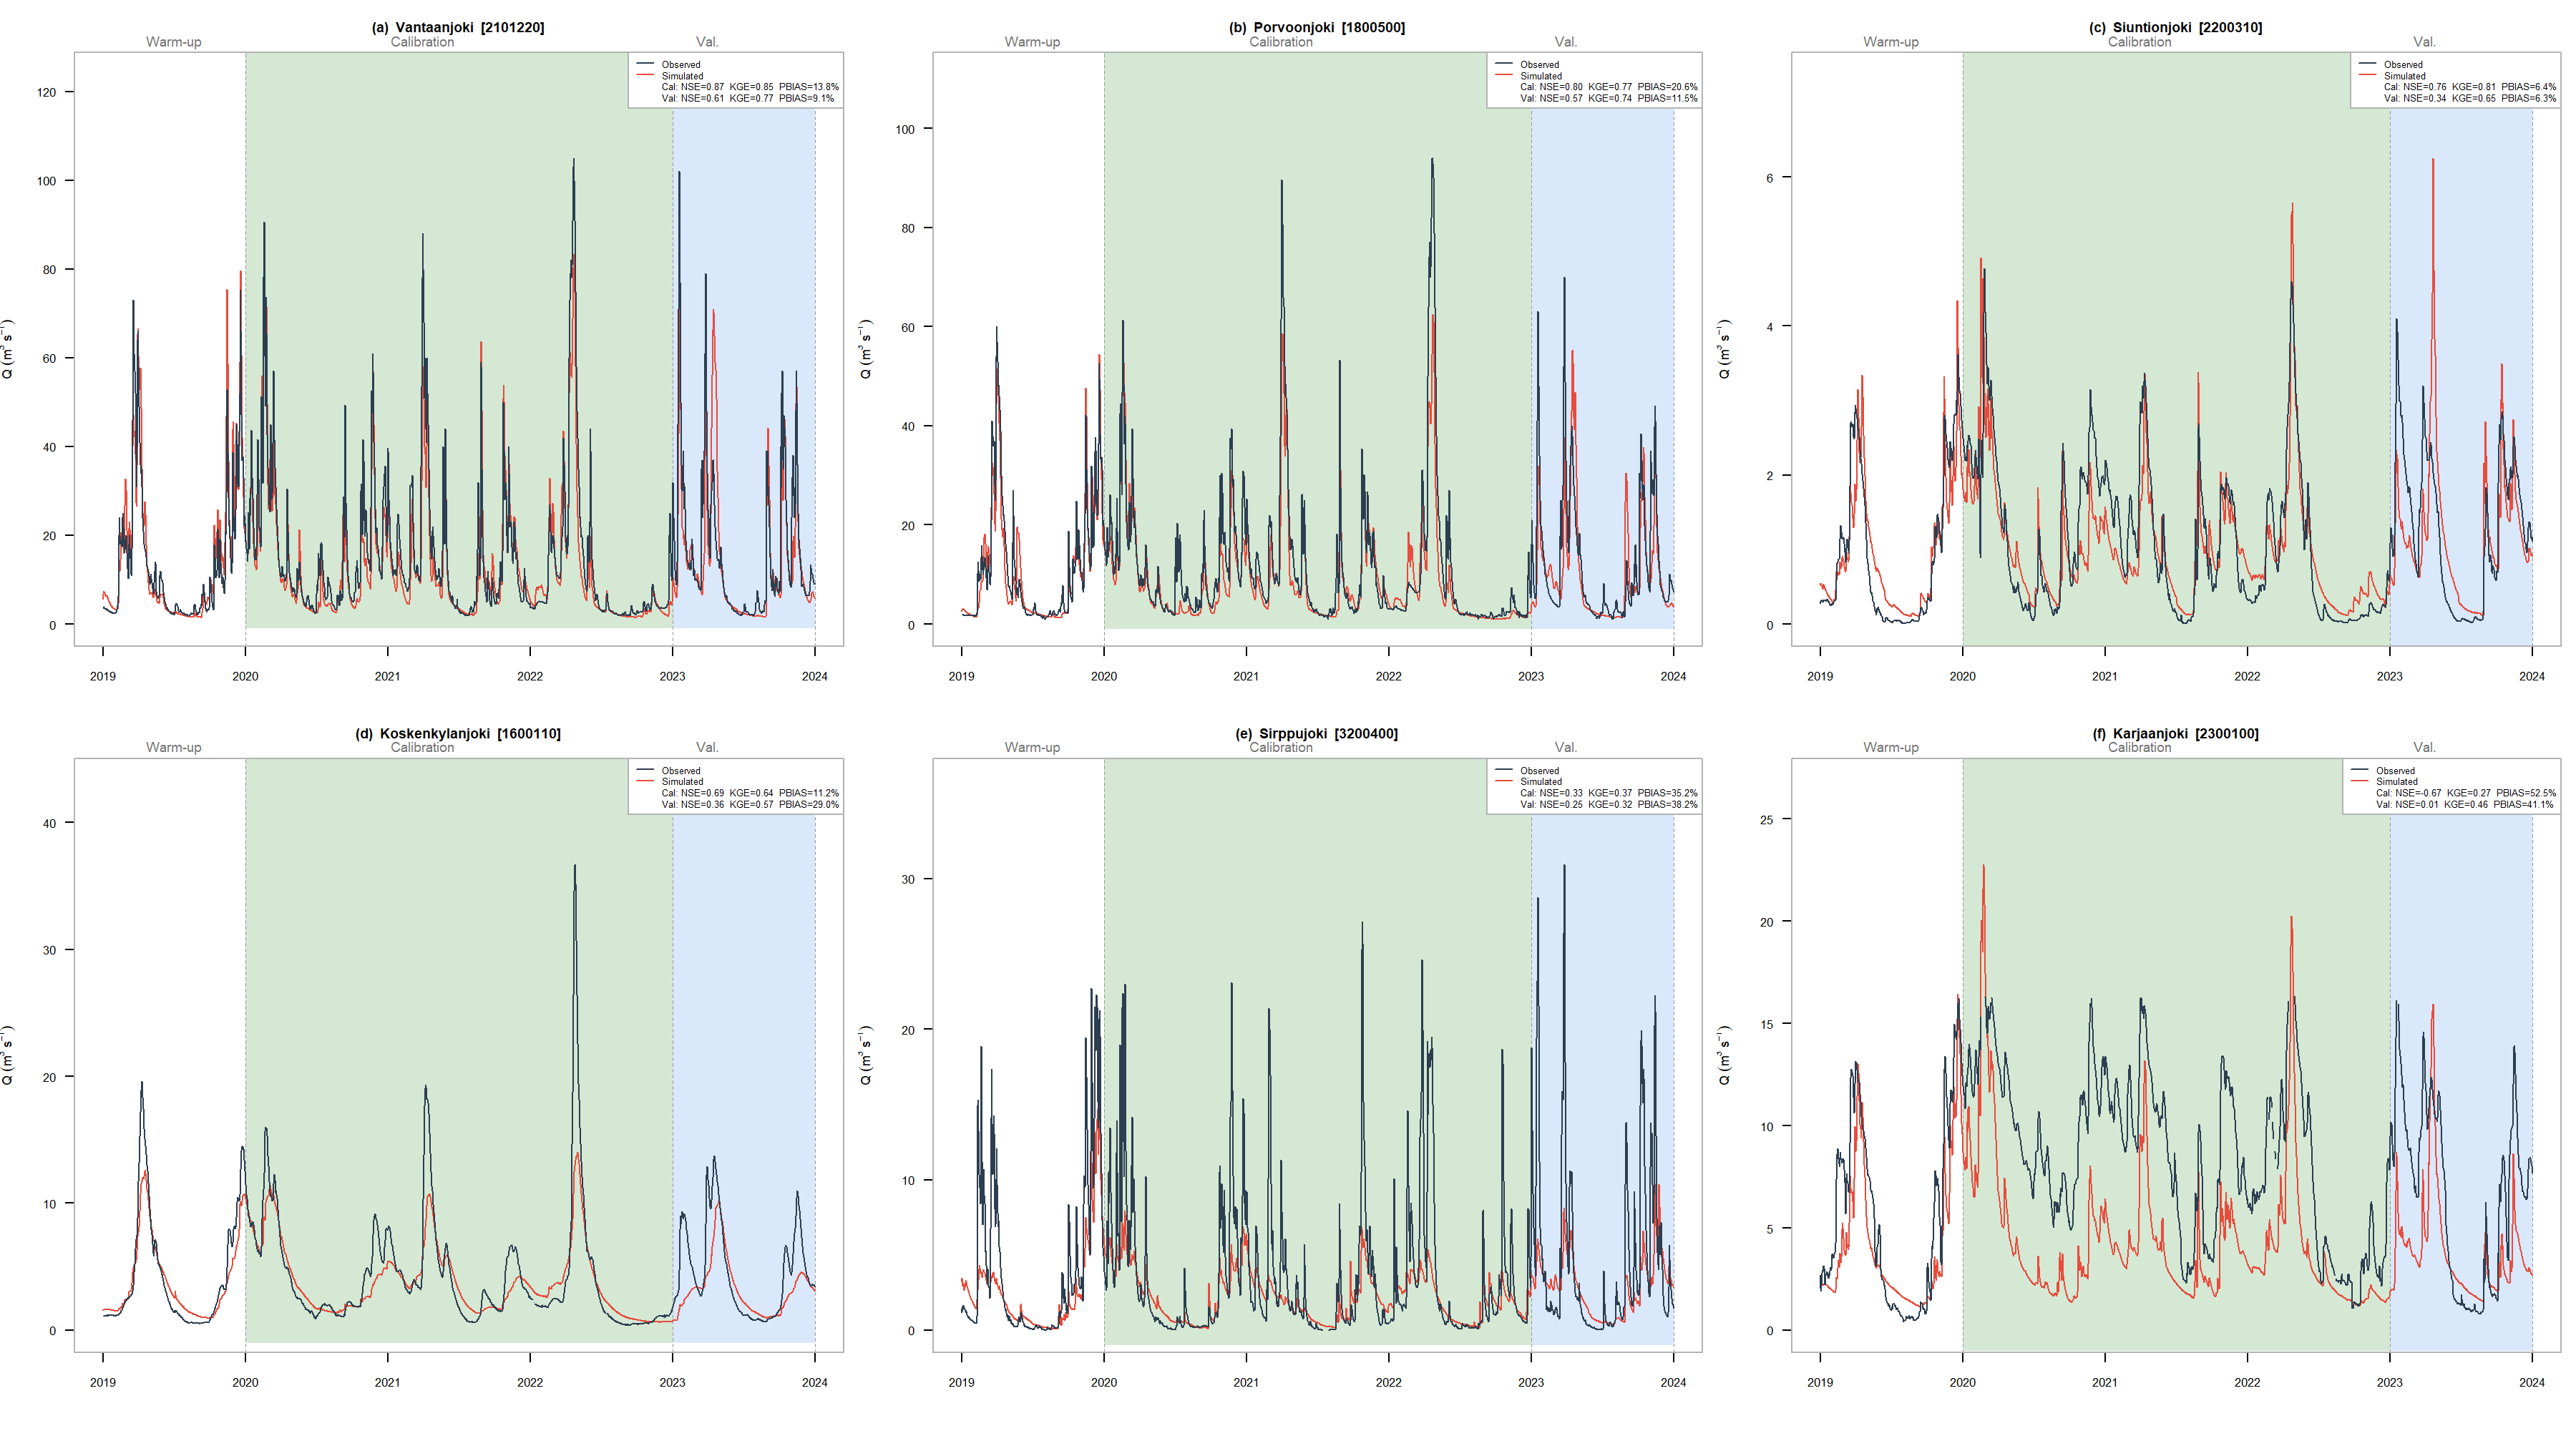
\includegraphics[width=0.95\textwidth]{figures_manuscript/fig01_hydrograph_compound}
\caption{Observed (dark) and simulated (red) daily discharge for six representative gauges covering the full range of calibration performance: (a) Vantaanjoki 2101220 (NSE\,=\,0.88); (b) Porvoonjoki 1800500 (NSE\,=\,0.82); (c) Siuntionjoki 2200310 (NSE\,=\,0.78); (d) Koskenkylanjoki 1600110 (NSE\,=\,0.75); (e) Sirppujoki 3200400 (NSE\,=\,0.42); (f) Karjaanjoki 2300340 (NSE\,=\,$-$0.76). Green shading = calibration period (2017--2022); blue shading = validation period (2023--2025). Metrics annotated for both periods. Panel (f) shows Karjaanjoki 2300340 rather than 2300100 as in an earlier draft: the corrected 2017--2022 calibration window (see Section~2.2.4) changes the ranking of worst-performing gauges, and 2300340 is now the true worst performer.}
\label{fig:hydrographs}
\end{figure}

\subsection{Seasonal freshwater availability}

Seasonal Q10 maps for the baseline period are presented in Figure~\ref{fig:seasonal_maps}. The spatial and seasonal patterns reveal strong heterogeneity across the study domain and a hydrological calendar in which summer and autumn low flows constitute the primary constraint on water availability for hydrogen production.

The regional median Q10 follows a pronounced seasonal cycle: spring (0.116\,m$^3$\,s$^{-1}$) $>$ winter (0.093\,m$^3$\,s$^{-1}$) $>$ annual (0.034\,m$^3$\,s$^{-1}$) $>$ summer (0.032\,m$^3$\,s$^{-1}$) $>$ autumn (0.028\,m$^3$\,s$^{-1}$). Autumn Q10 is the lowest of all seasons — a counterintuitive finding explained by the persistence of summer drought conditions into September before autumn recharge has propagated through the soil-groundwater-stream system. The proportion of subcatchments below the indicative 0.05\,m$^3$\,s$^{-1}$ threshold ranges from 28.5\% in spring to 60.8\% in autumn (Table~\ref{tab:q10_summary}).

A clear west-to-east gradient characterises baseline summer Q10. Western catchments (Sirppujoki, Hirvijoki, Mynajoki, Aurajoki, Uskelanjoki) are dominated by low Q10 values, reflecting their small drainage areas, high agricultural land cover, clay-dominated soils with limited aquifer storage capacity, and absence of significant lake buffering. The P10--P90 range of summer Q10 across all subcatchments spans more than three orders of magnitude (0.000 to 0.525\,m$^3$\,s$^{-1}$), confirming that location-specific analysis is essential and regional averages are uninformative for site screening.

Winter Q10 is notably higher than summer Q10 (32.6\% of subcatchments below threshold in winter vs 58.5\% in summer), demonstrating that groundwater-fed baseflow sustains winter low flows more reliably than the evapotranspiration-depleted summer baseflows. Peatland-dominated subcatchments in the western region show relatively high winter Q10 compared to their summer values, consistent with the known function of peatlands as hydrological buffers that release stored water slowly throughout the cold season.

\begin{figure}[htbp]
\centering
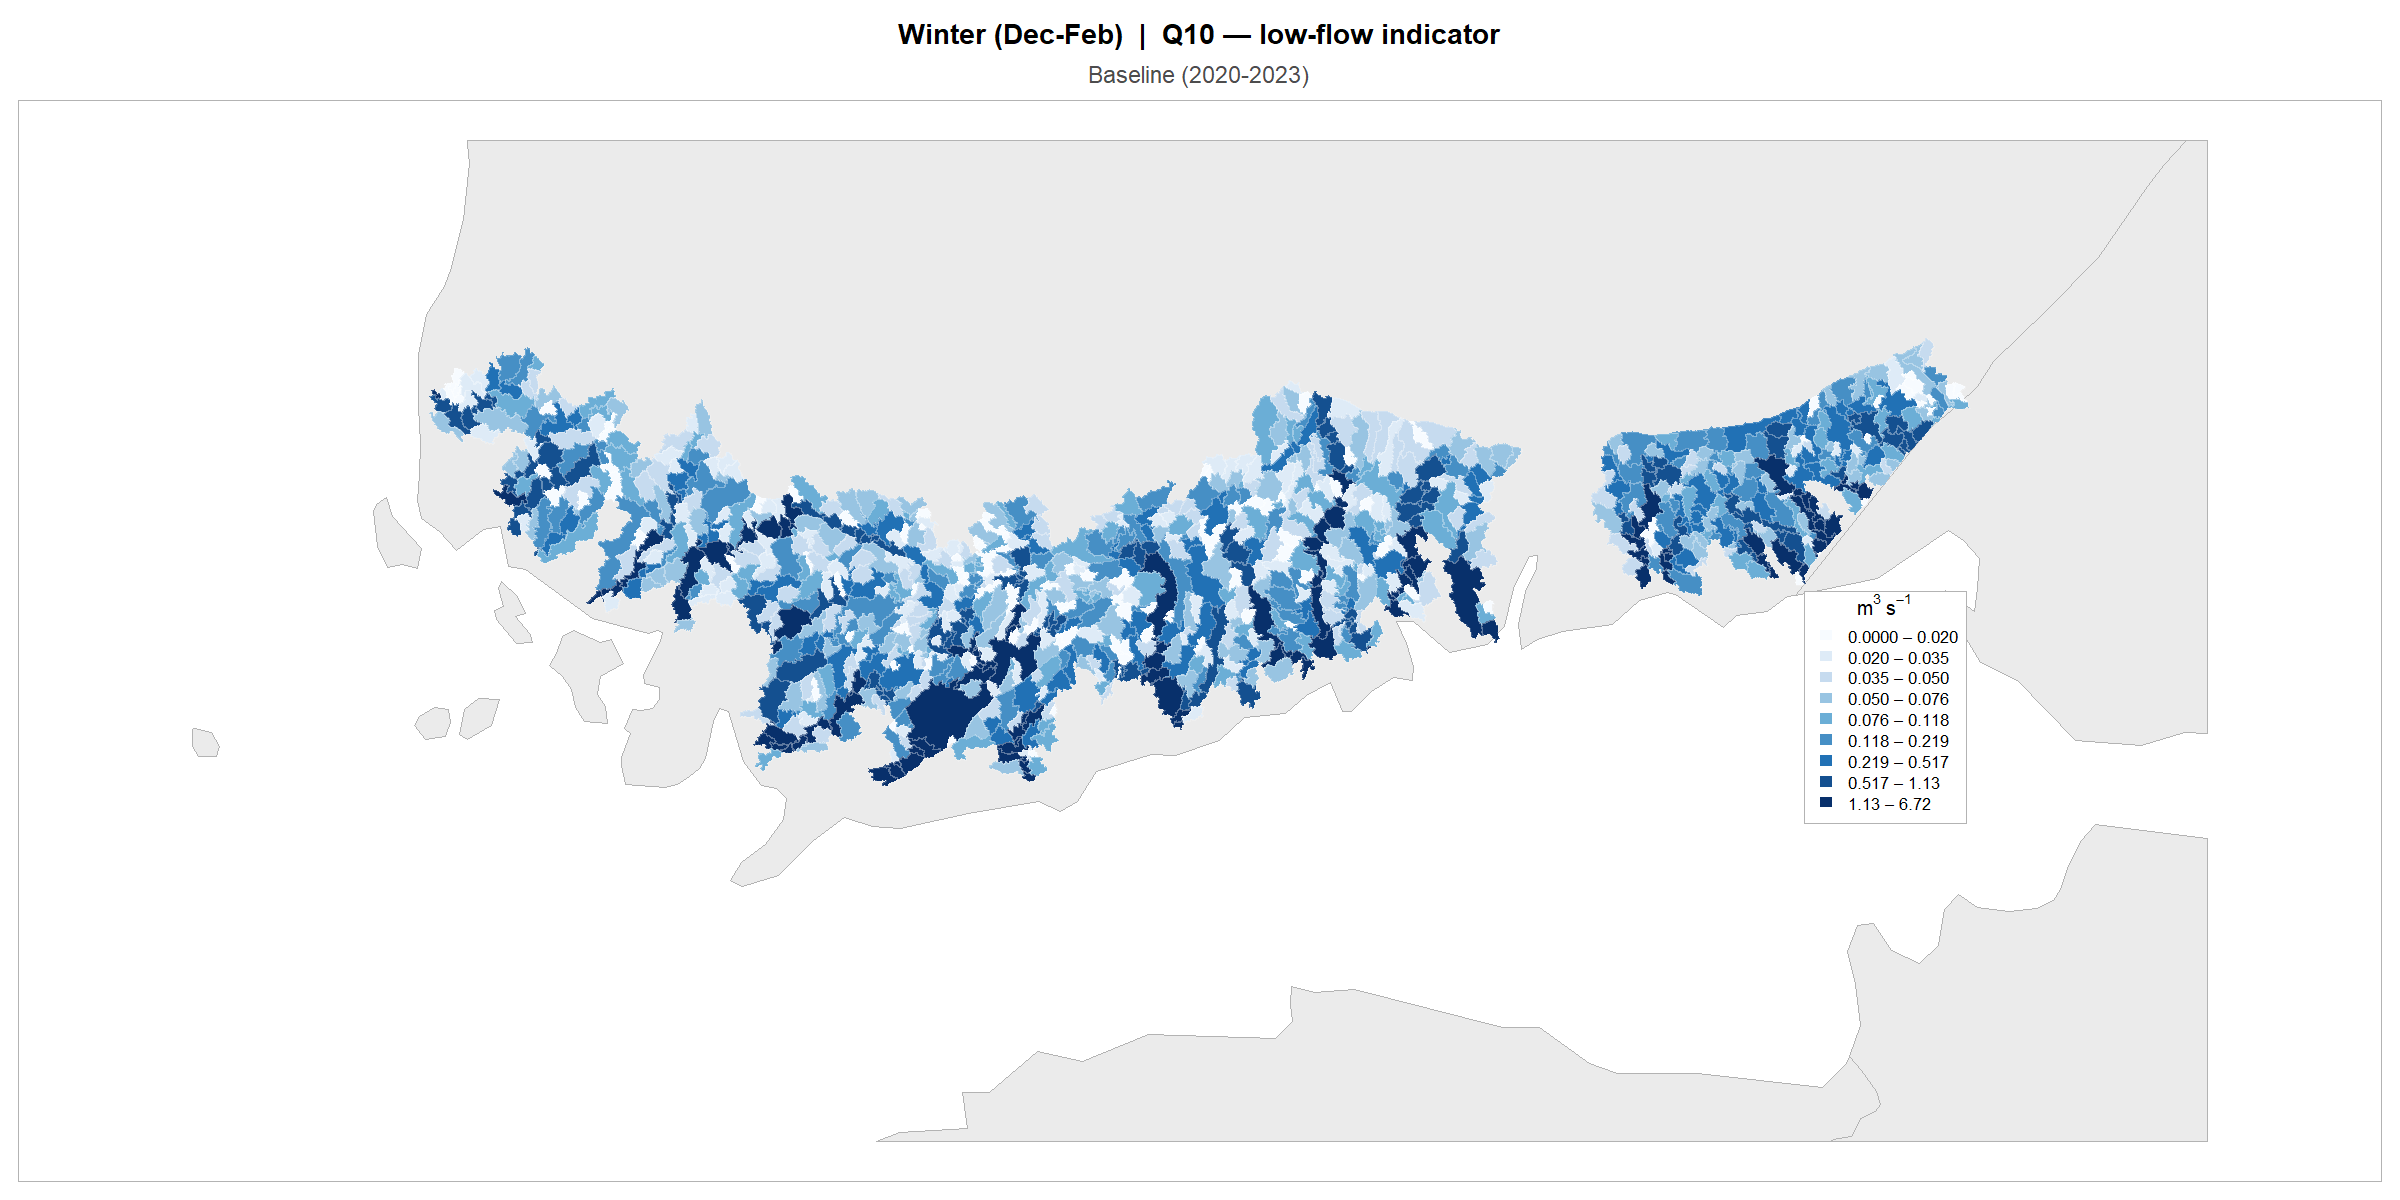
\includegraphics[width=0.75\textwidth]{figures_manuscript/fig02_baseline_winter_q10}\\[4pt]
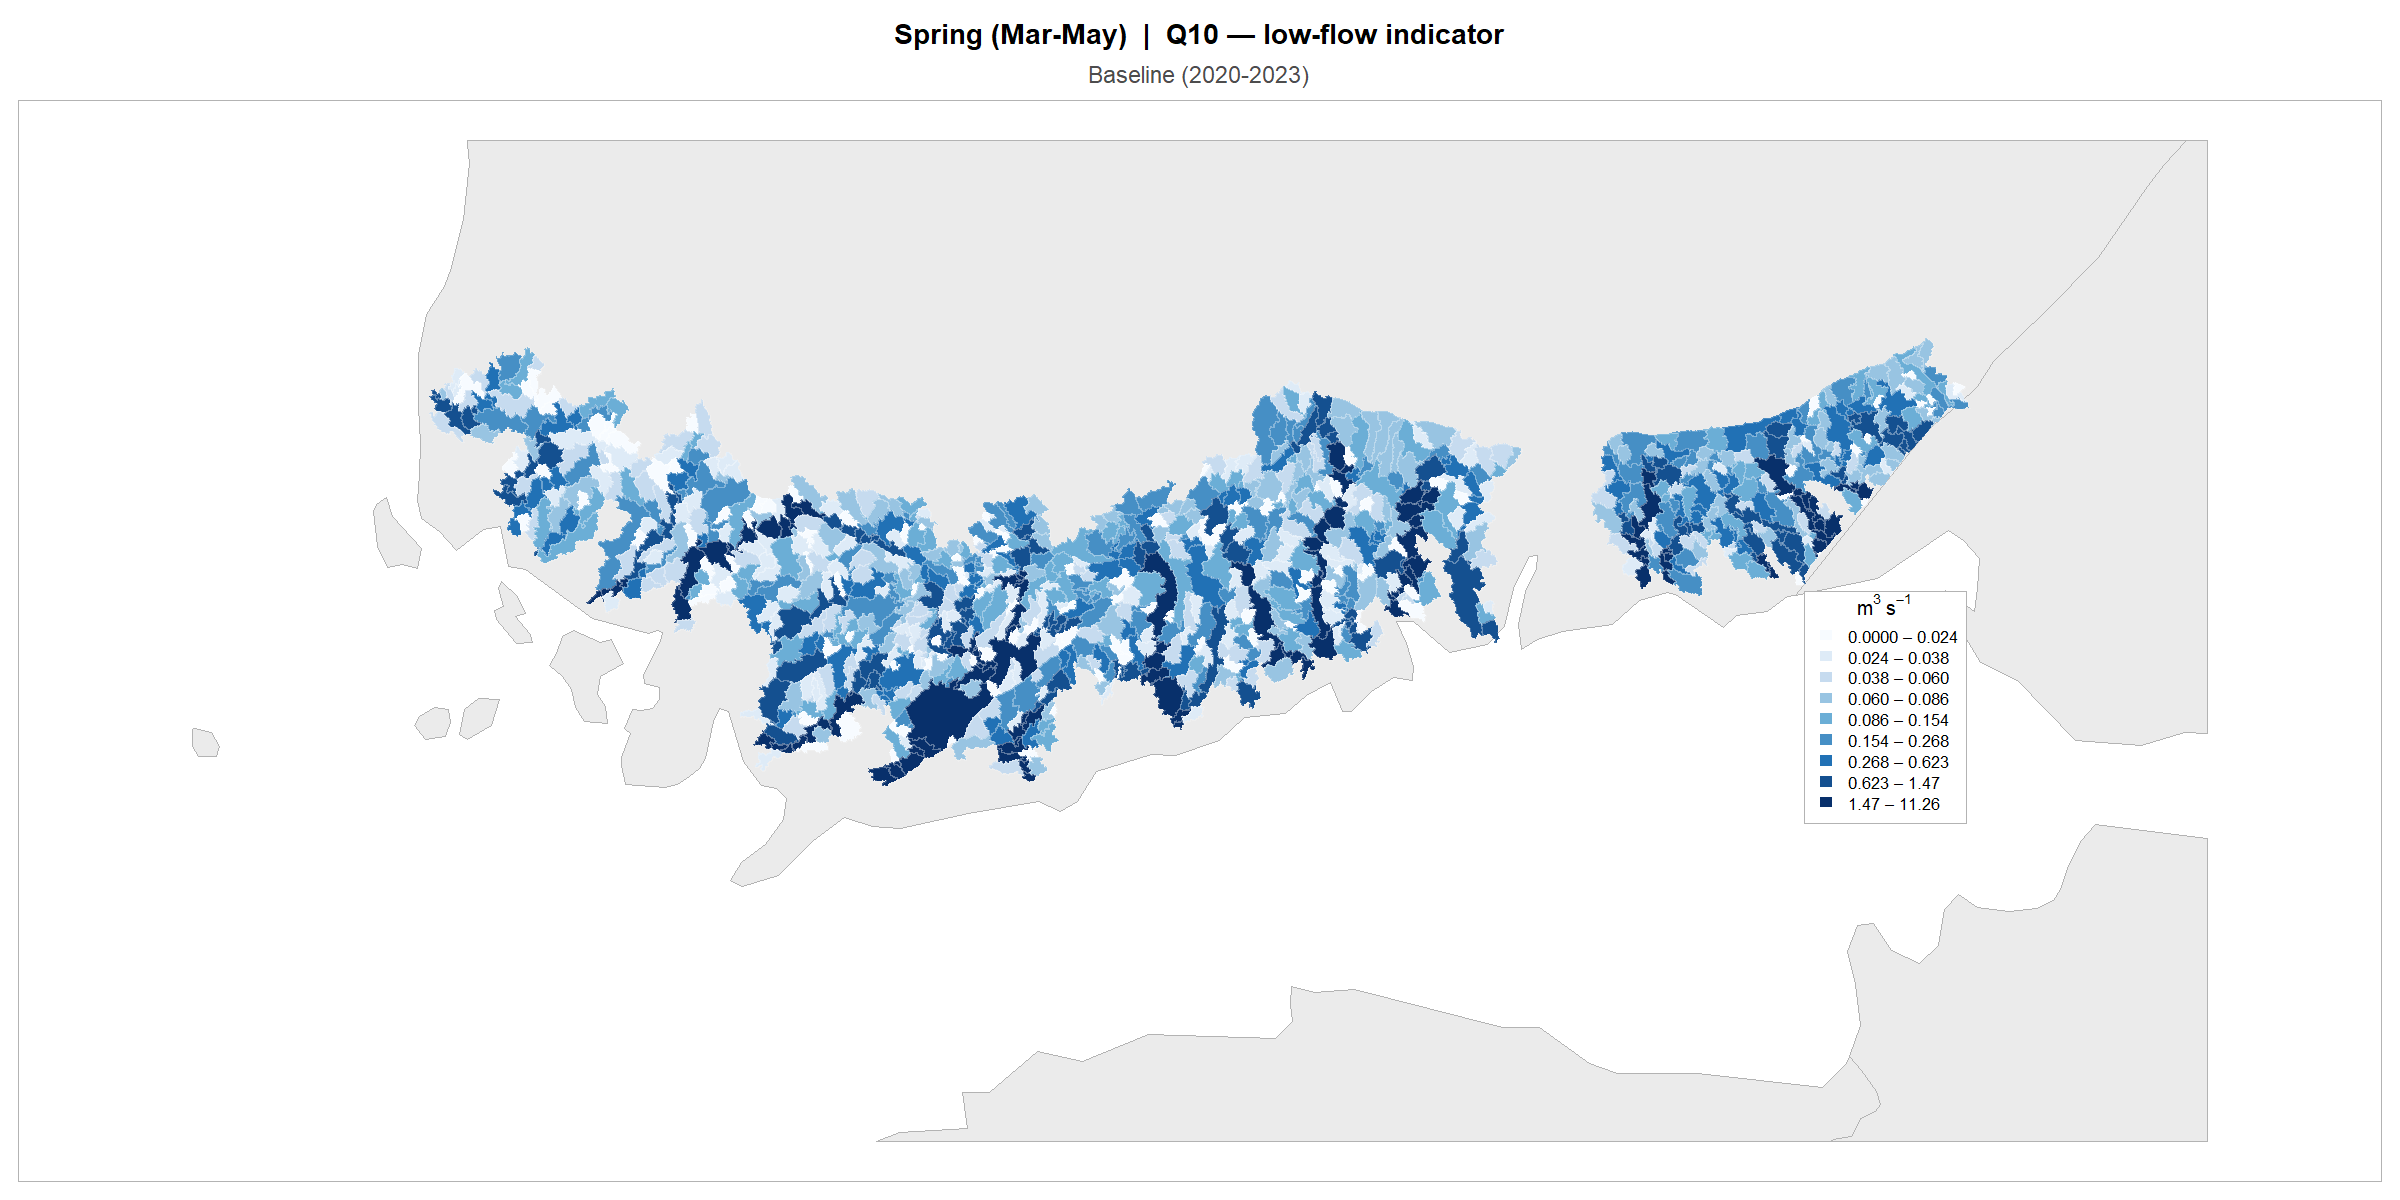
\includegraphics[width=0.75\textwidth]{figures_manuscript/fig02_baseline_spring_q10}\\[4pt]
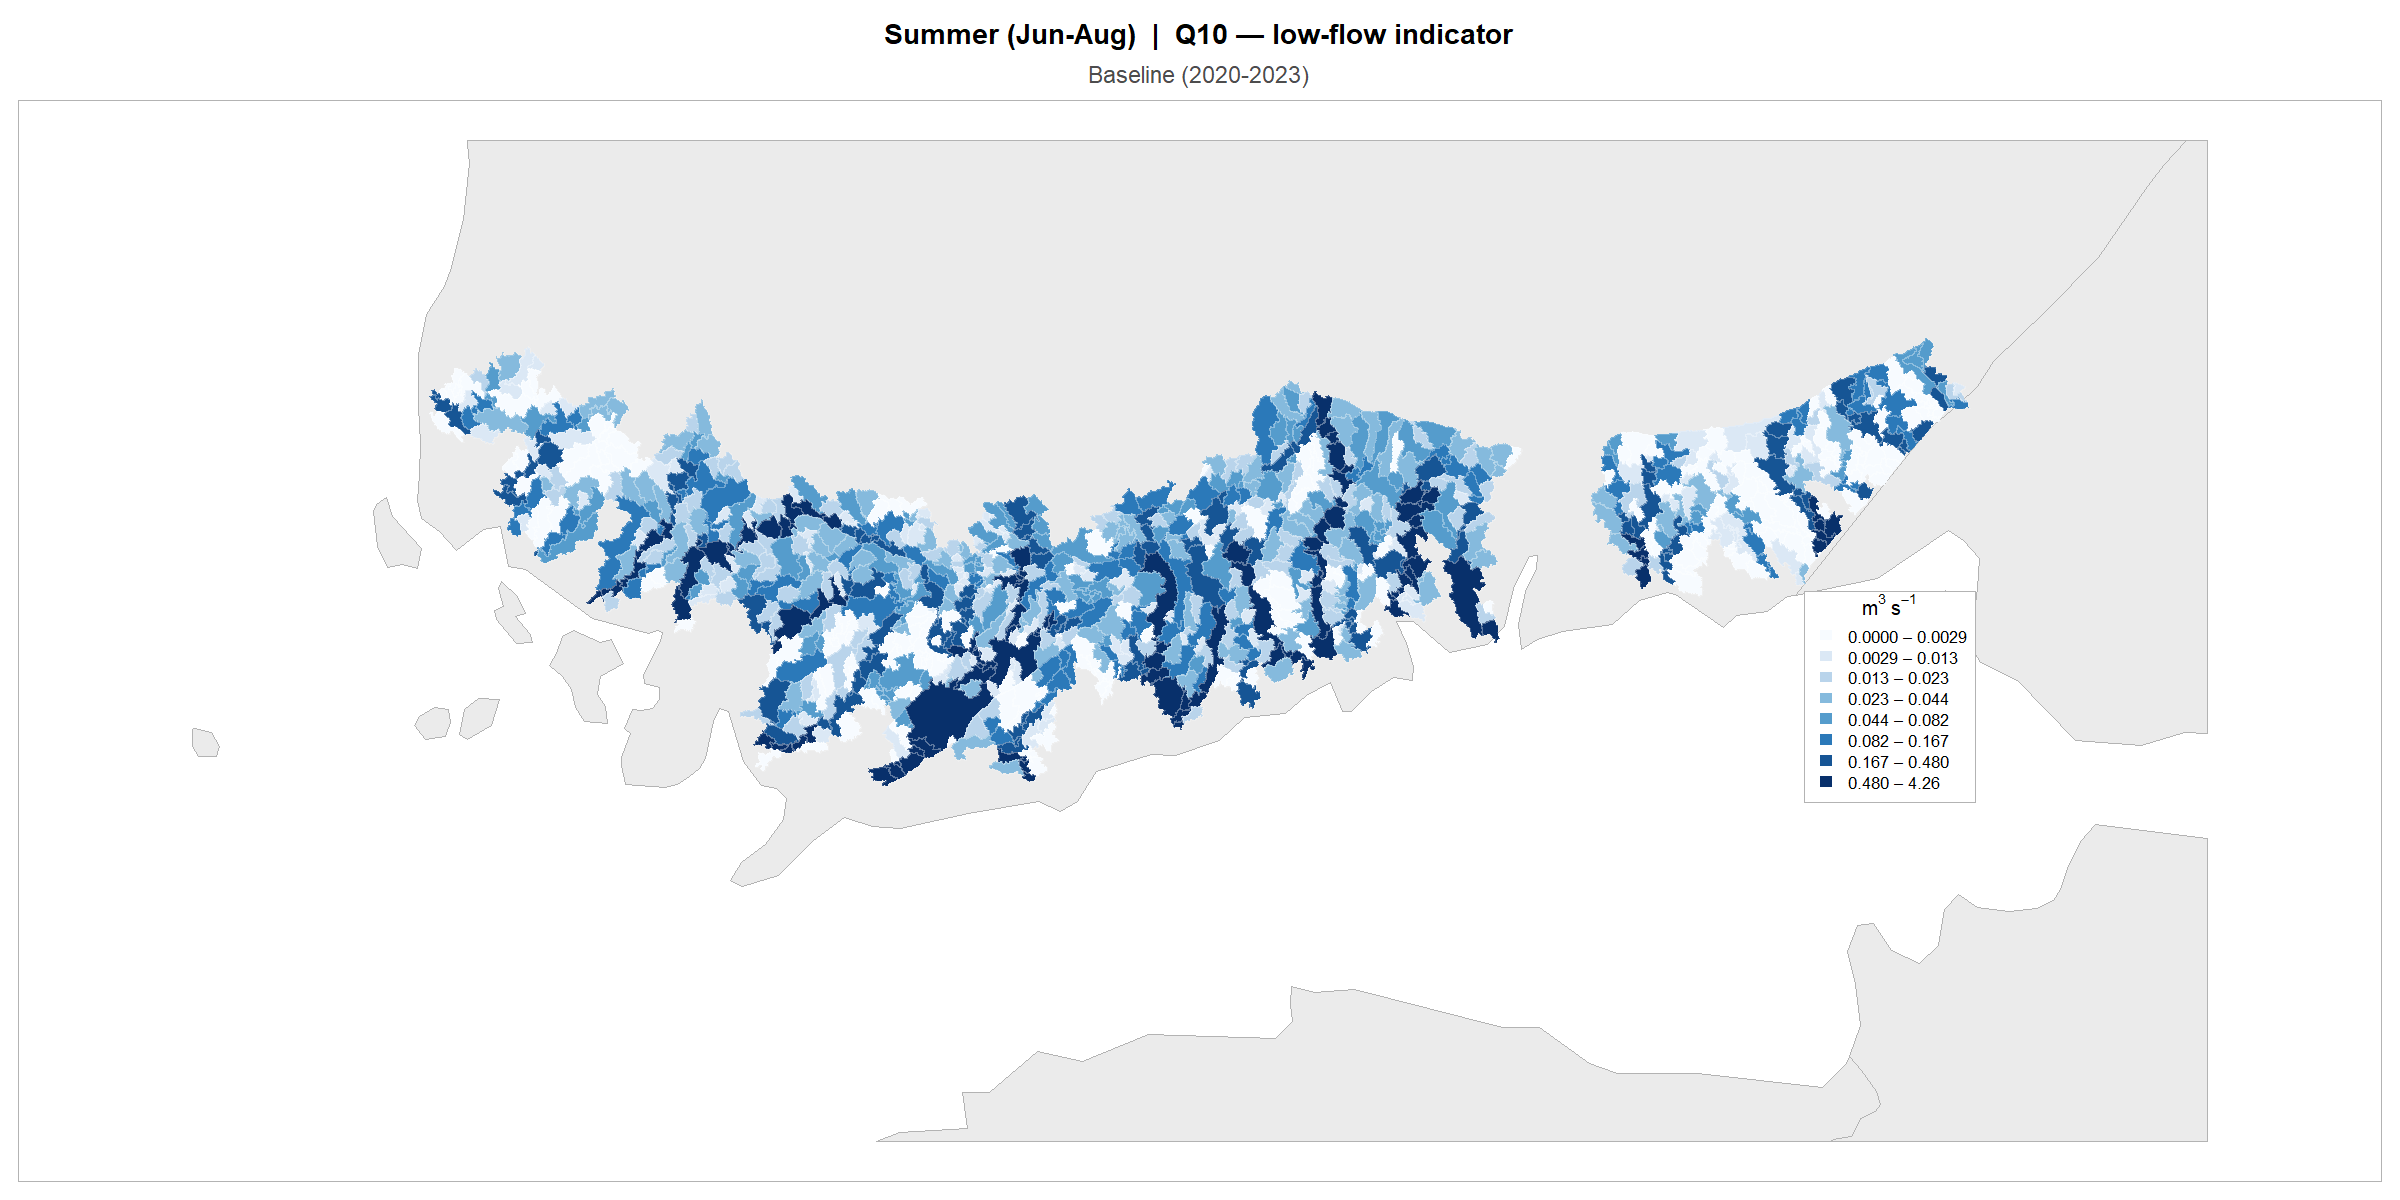
\includegraphics[width=0.75\textwidth]{figures_manuscript/fig02_baseline_summer_q10}\\[4pt]
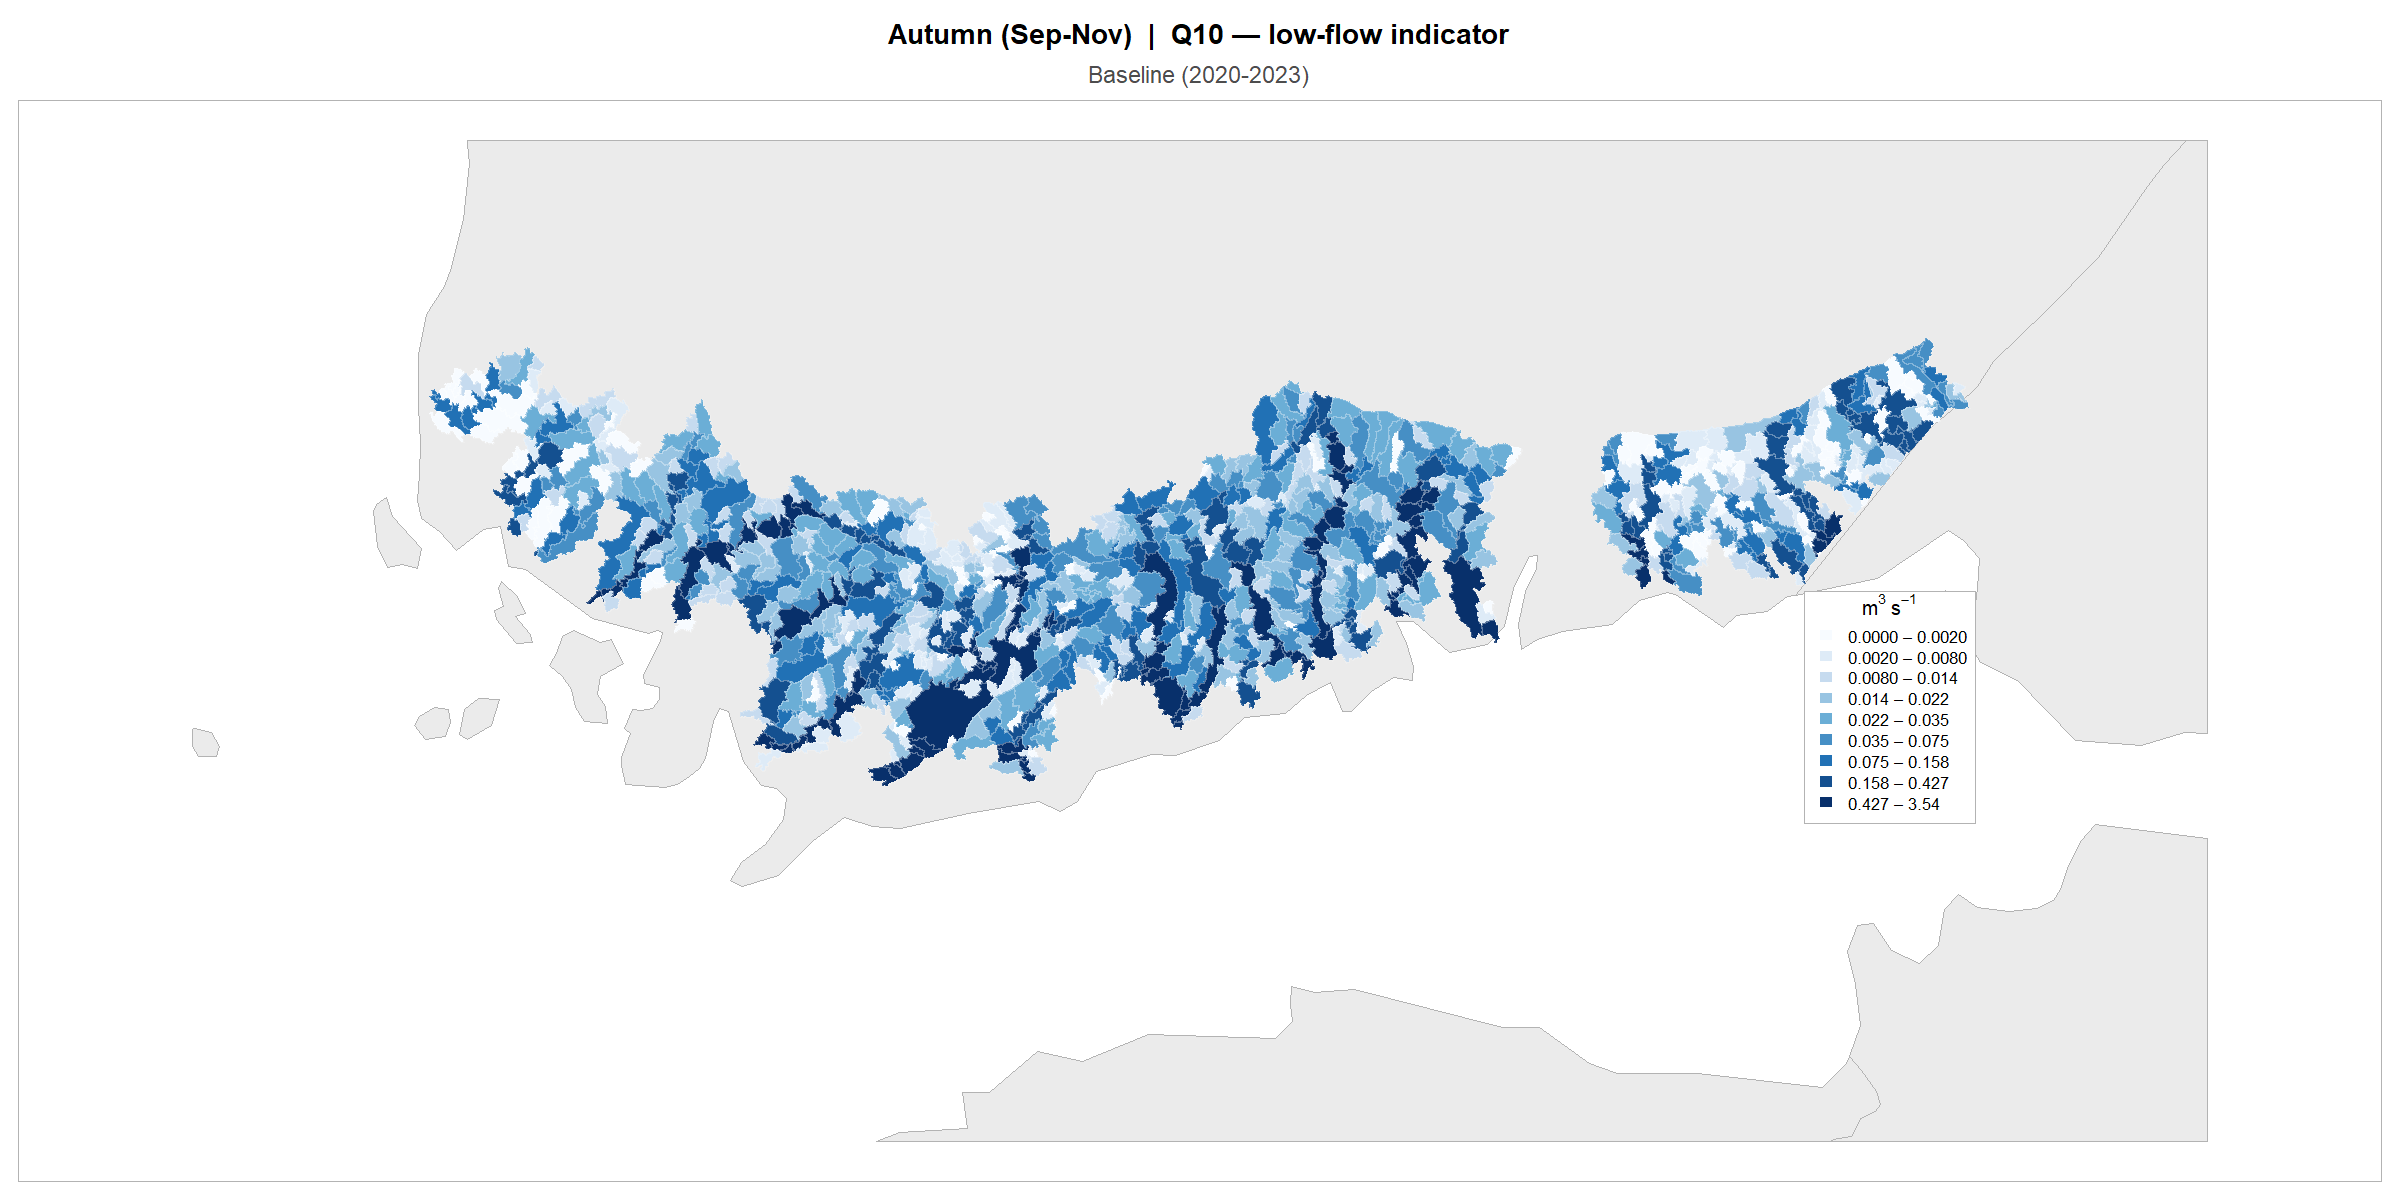
\includegraphics[width=0.75\textwidth]{figures_manuscript/fig02_baseline_autumn_q10}
\caption{Baseline seasonal Q10 discharge (m$^3$\,s$^{-1}$) across 1,158 subcatchments in southern Finland for (top to bottom) winter (December--February), spring (March--May), summer (June--August), and autumn (September--November). Colour scale uses quantile-based classification; light blue = low, dark blue = high discharge.}
\label{fig:seasonal_maps}
\end{figure}

\begin{table}[htbp]
\caption{Regional Q10 summary statistics by season for the baseline scenario across all 1,158 subcatchments. P10 and P90 are the 10th and 90th percentiles across subcatchments. N$_{<0.05}$ and \% $_{<0.05}$ indicate the number and proportion of subcatchments below the indicative industrial abstraction threshold of 0.05\,m$^3$\,s$^{-1}$.}
\label{tab:q10_summary}
\small
\begin{tabular}{lrrrrr}
\toprule
Season & Median Q10 & P10 Q10 & P90 Q10 & N$_{<0.05}$ & \%$_{<0.05}$ \\
 & (m$^3$\,s$^{-1}$) & (m$^3$\,s$^{-1}$) & (m$^3$\,s$^{-1}$) & & \\
\midrule
Winter (Dec--Feb) & 0.093 & 0.019 & 1.229 & 378 & 32.6 \\
Spring (Mar--May) & 0.116 & 0.023 & 1.675 & 330 & 28.5 \\
Summer (Jun--Aug) & 0.032 & 0.000 & 0.525 & 677 & 58.5 \\
Autumn (Sep--Nov) & 0.028 & 0.001 & 0.500 & 704 & 60.8 \\
Annual            & 0.034 & 0.001 & 0.620 & 667 & 57.6 \\
\bottomrule
\end{tabular}
\end{table}

\subsection{Climate change scenario effects}

The SSP2-4.5 climate scenario produces opposing seasonal effects on Q10 that are critical for hydrogen production planning (Figures~\ref{fig:delta_summer} and~\ref{fig:delta_winter}). Summer and autumn Q10 decrease substantially and near-universally, while winter Q10 increases across much of the domain.

For summer Q10, 98.7\% of subcatchments show a decrease under the climate scenario, with a regional median change of $-24.4\%$ (P10: $-82.6\%$, P90: $-10.0\%$). The mechanism is straightforward: temperature increases of $+2.3$ to $+3.2\,^\circ$C drive substantially higher evapotranspiration throughout the growing season, depleting soil moisture reserves that would otherwise recharge groundwater and sustain summer baseflows. The slight decrease in July precipitation ($-1\%$) amplifies this effect. The spatial pattern of summer Q10 decline is not uniform — the western catchments already experiencing the lowest baseline flows show the largest relative decreases, intensifying the existing spatial gradient. This ``droughts get drier'' dynamic means that the areas already most constrained under current conditions become increasingly infeasible for surface water-based hydrogen production under future climate.

For winter Q10, the climate scenario produces widespread increases reflecting the shift from snowfall to rainfall under warmer winter temperatures. More precipitation falling directly as rain generates immediate runoff and groundwater recharge rather than accumulating in snowpack, increasing winter baseflows. This creates a seasonally opposing trend: future climate simultaneously relaxes the winter water constraint while tightening the summer constraint.

\subsection{Urban growth scenario effects}

The urban growth scenario exerts a negligible regional signal on summer Q10 relative to climate change (Table~\ref{tab:delta_summary}). The regional median change in summer Q10 is $-0.43\%$ (compared to $-24.4\%$ for climate), and only 53.8\% of subcatchments show any decrease (compared to 98.7\% for climate). Climate change outweighs urban growth as a driver of summer low-flow change by approximately 57:1 in terms of median regional impact.

The modest decreases in urbanising subcatchments reflect reduced groundwater recharge from increased impervious cover, which reduces infiltration and therefore baseflow. The largest urban growth effects are concentrated in the Vantaanjoki catchment (Helsinki metropolitan area), where urban fractions increase most strongly under the Statistics Finland projections, but even here the absolute magnitude of the Q10 change is small relative to the climate signal.

The combined scenario — applying both climate forcing changes and urban land cover modifications simultaneously — is nearly indistinguishable from the climate-only scenario in summer (median $-26.0\%$ vs $-24.4\%$). This confirms that at the regional scale, urban growth is a secondary modifier of the climate change signal rather than an independent driver of water scarcity for hydrogen production.

\begin{figure}[htbp]
\centering
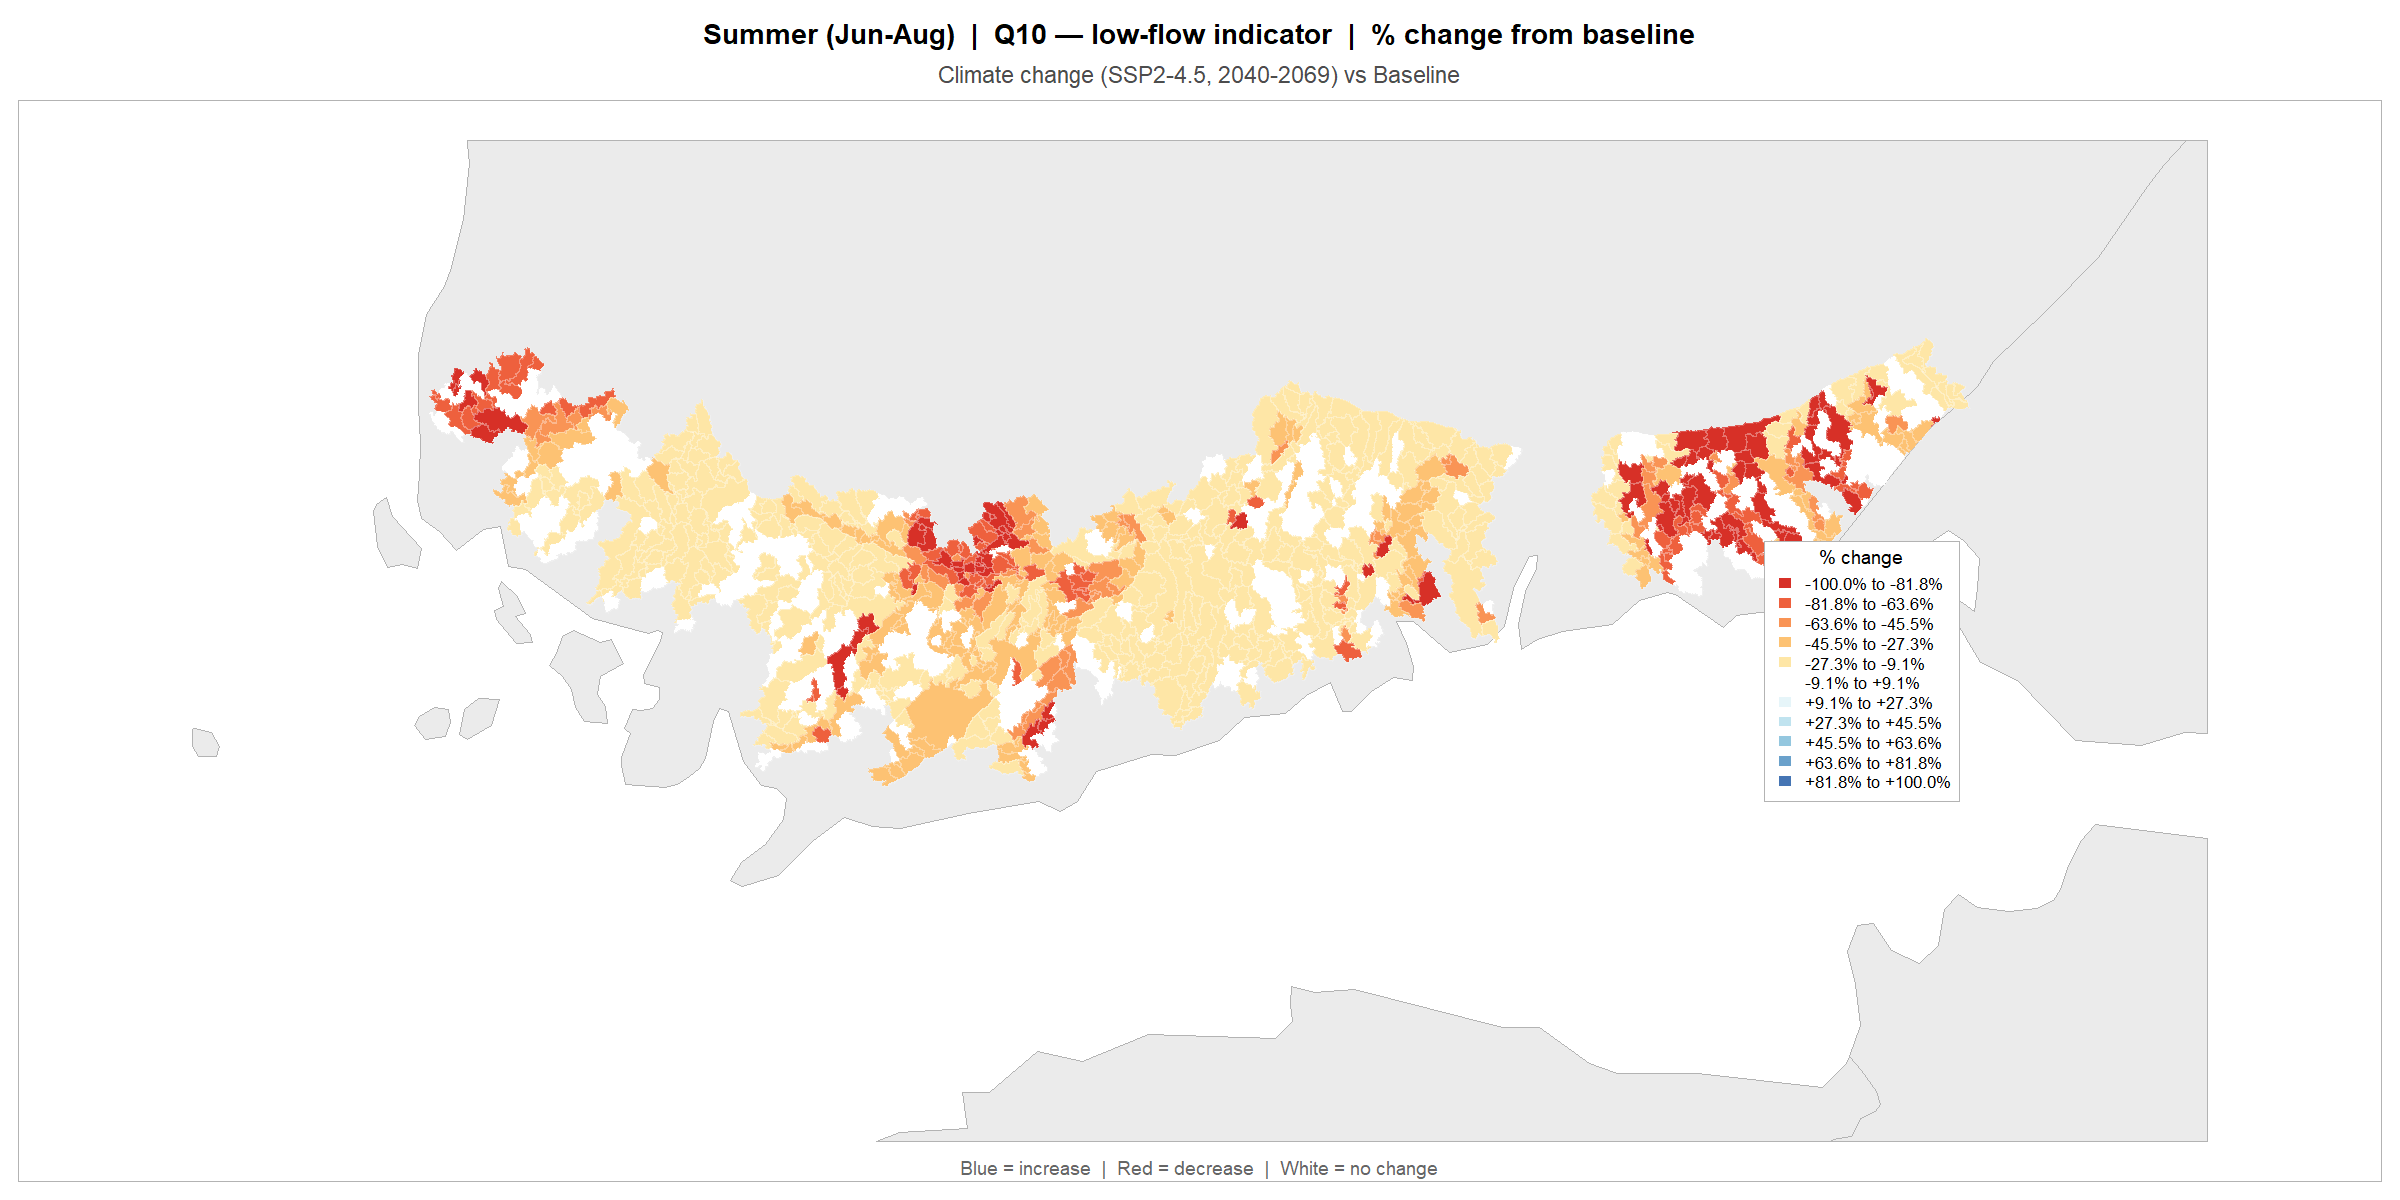
\includegraphics[width=0.80\textwidth]{figures_manuscript/fig03_climate_summer_q10_delta}\\[4pt]
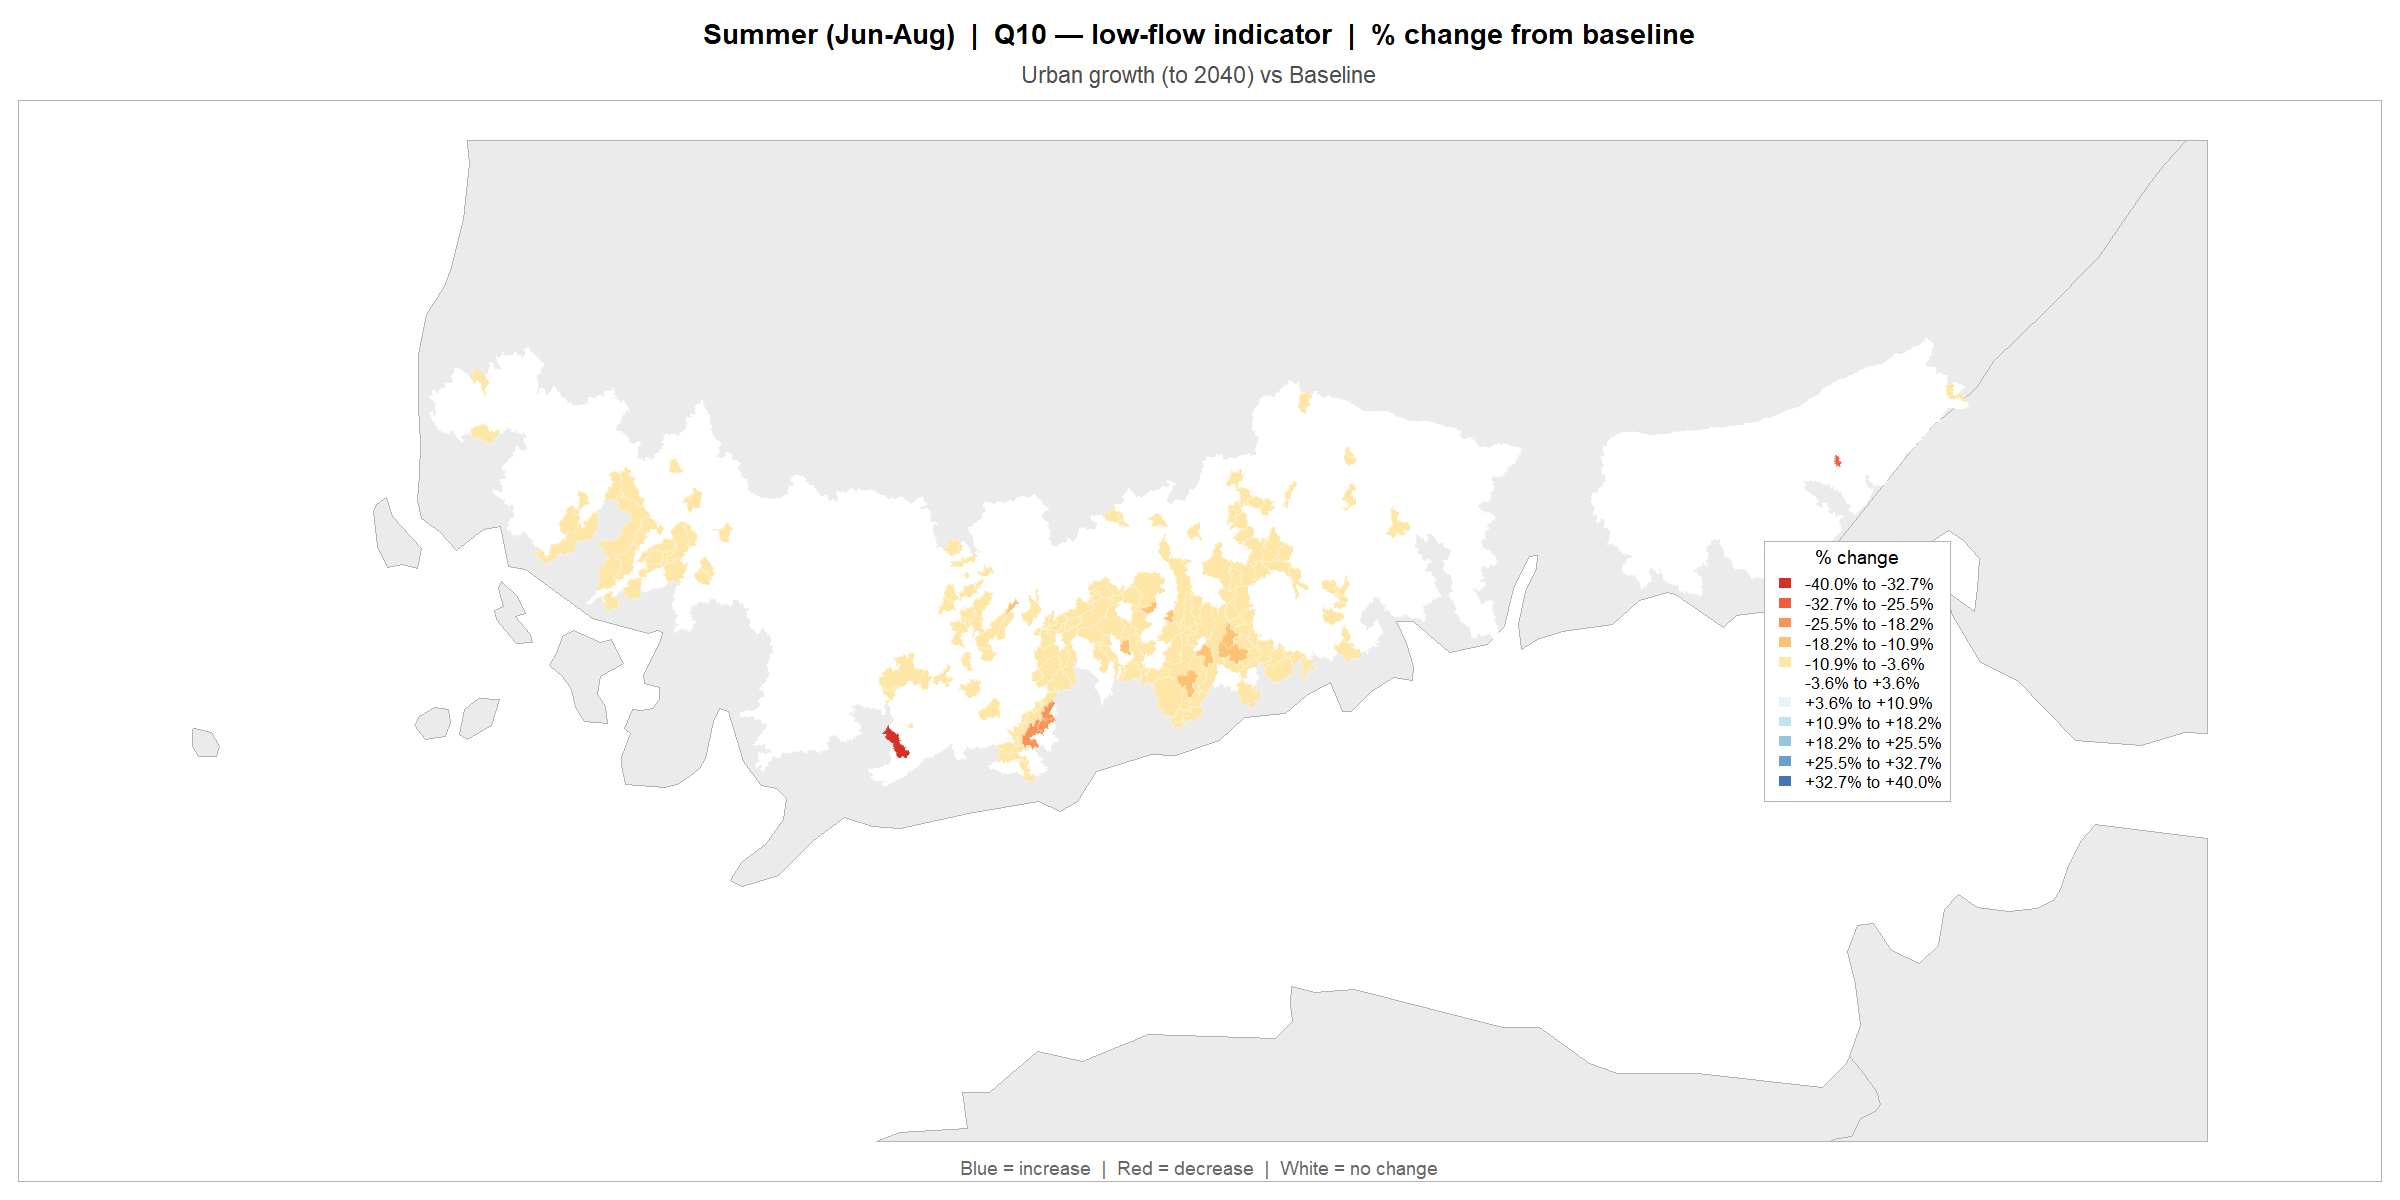
\includegraphics[width=0.80\textwidth]{figures_manuscript/fig03_urban_summer_q10_delta}\\[4pt]
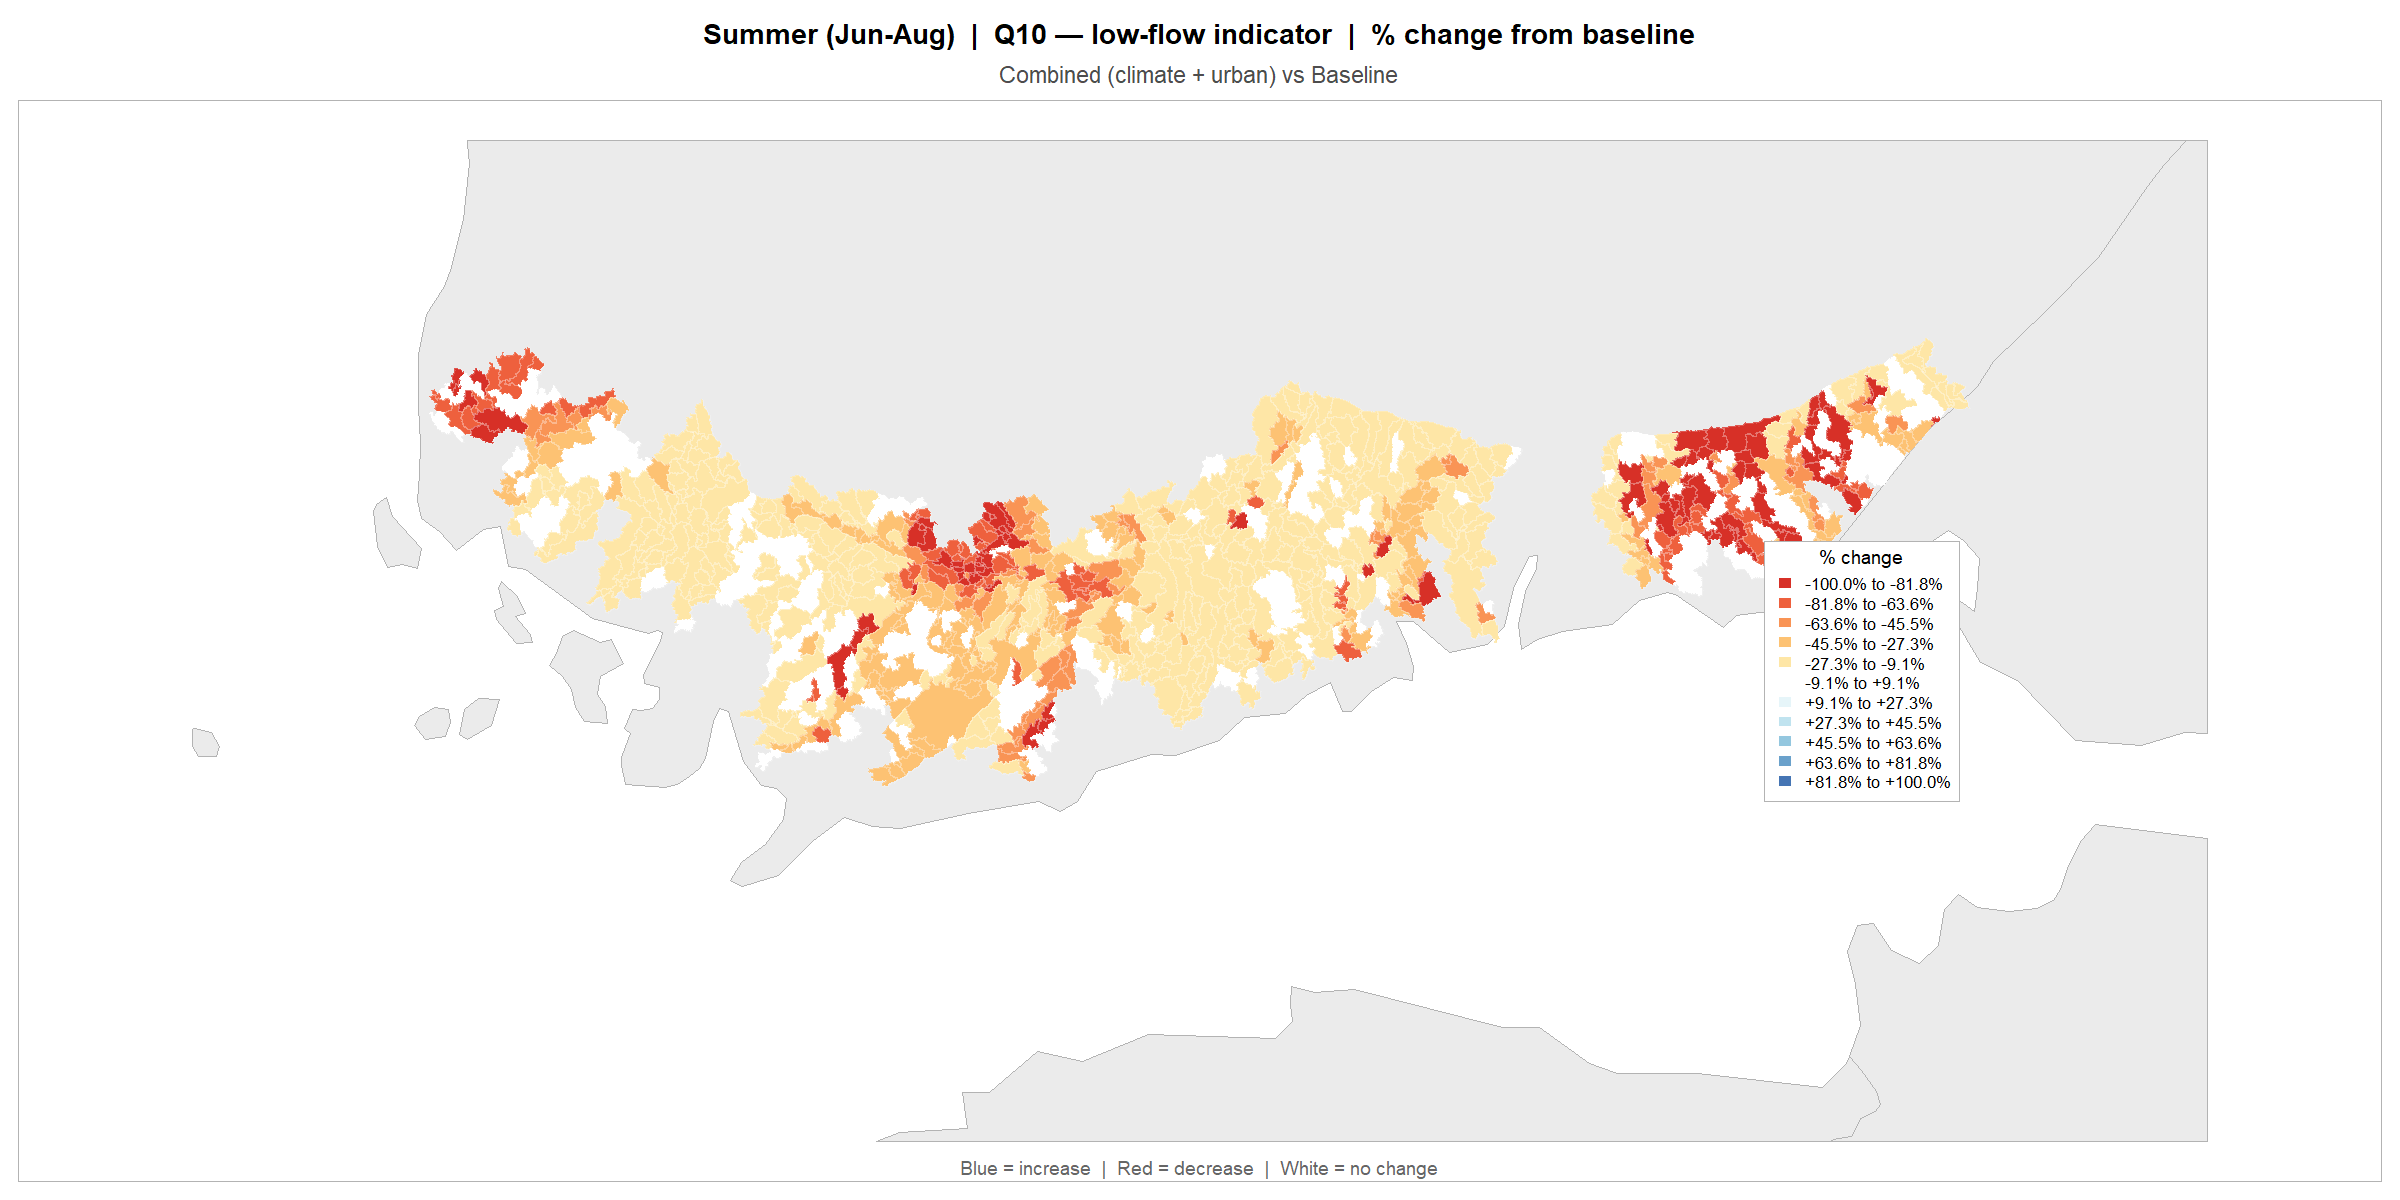
\includegraphics[width=0.80\textwidth]{figures_manuscript/fig03_combined_summer_q10_delta}
\caption{Percentage change in summer Q10 from baseline for (top) climate change (SSP2-4.5, 2040--2069), (middle) urban growth (to 2040), and (bottom) combined scenarios. Blue = increase; red = decrease; white = no change; grey = undefined (baseline Q10 = 0). Note the contrasting magnitude of change between climate ($-$24.4\% median) and urban ($-$0.43\% median) scenarios.}
\label{fig:delta_summer}
\end{figure}

\begin{figure}[htbp]
\centering
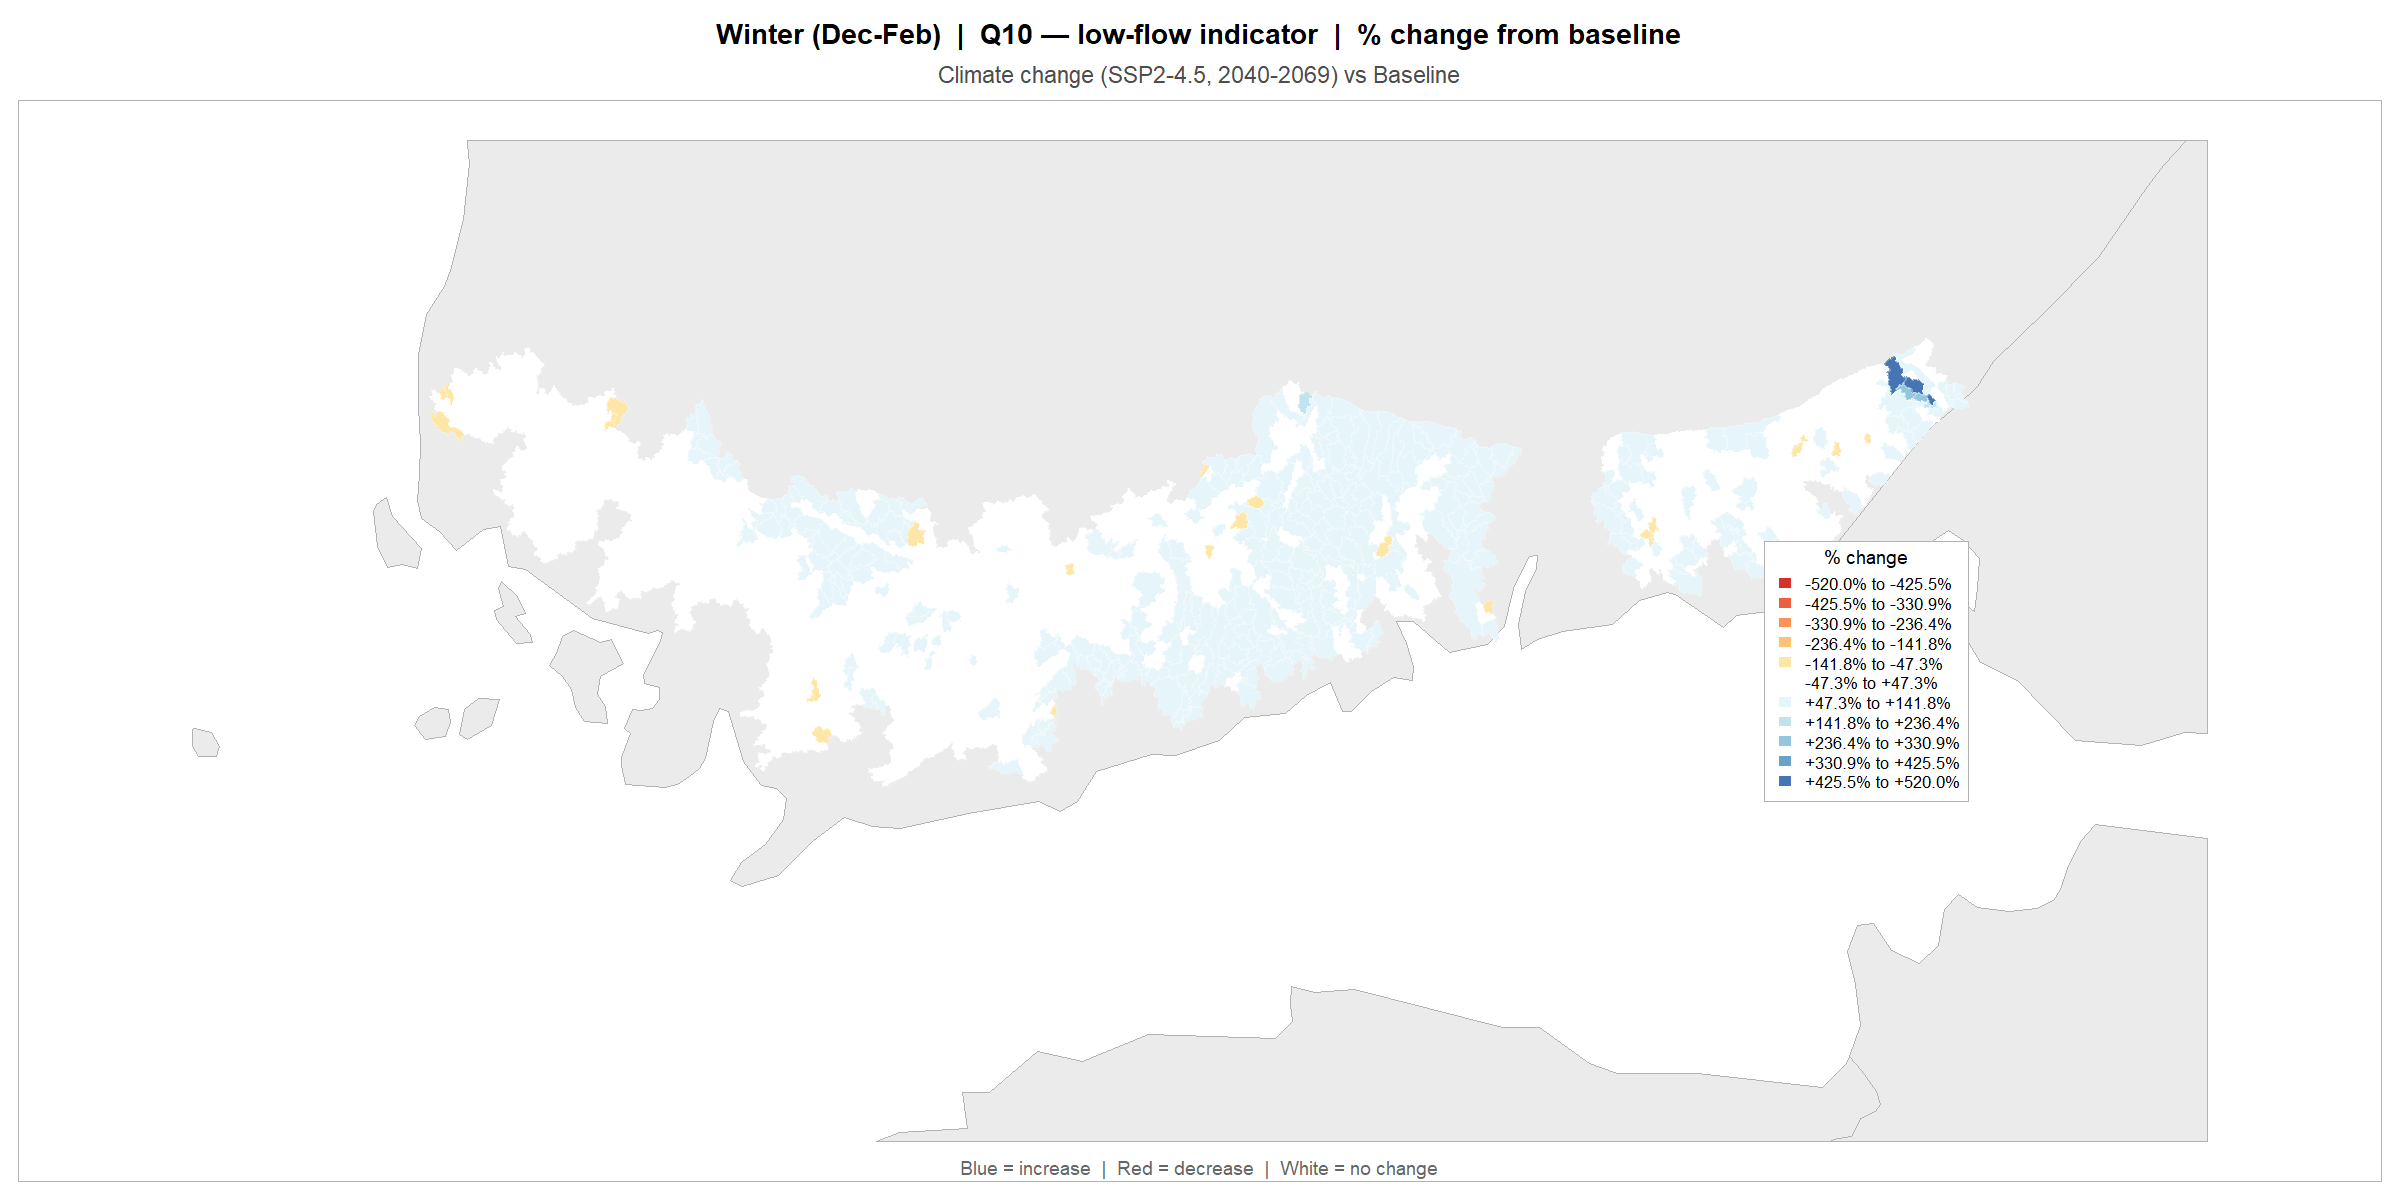
\includegraphics[width=0.80\textwidth]{figures_manuscript/fig04_climate_winter_q10_delta}
\caption{Percentage change in winter Q10 from baseline under the climate change scenario (SSP2-4.5, 2040--2069). Widespread increases in winter Q10 reflect the shift from snowfall to rainfall under warmer winter temperatures, creating an opposing seasonal trend to the summer Q10 decrease shown in Figure~\ref{fig:delta_summer}.}
\label{fig:delta_winter}
\end{figure}

\begin{table}[htbp]
\caption{Summer Q10 percentage change from baseline by scenario. Statistics computed across subcatchments with non-zero baseline summer Q10. P10 and P90 are the 10th and 90th percentiles of the percentage change distribution. \%\,decrease = proportion of subcatchments showing any reduction in summer Q10.}
\label{tab:delta_summary}
\small
\begin{tabular}{lrrrr}
\toprule
Scenario & Median change (\%) & P10 (\%) & P90 (\%) & \% decrease \\
\midrule
Climate change (SSP2-4.5) & $-$24.4 & $-$82.6 & $-$10.0 & 98.7 \\
Urban growth              &  $-$0.4 &  $-$5.6 &   $+$0.0 & 53.8 \\
Combined                  & $-$26.0 & $-$83.2 & $-$11.9 & 98.8 \\
\bottomrule
\end{tabular}
\end{table}

Based on the hydrological results, three broad tiers of water availability for surface water-based hydrogen production can be identified across the study domain:

\textit{Most suitable — eastern catchments.} Koskenkylanjoki, Porvoonjoki, Taasianjoki, Vehkajoki, Urpalanjoki, and Juustilanjoki have the highest summer and annual Q10 values, the largest drainage areas providing hydrological buffering, and are less severely affected by the climate scenario. These catchments represent the strongest candidates for direct surface water abstraction for hydrogen production.

\textit{Conditionally suitable — central catchments.} Vantaanjoki, Mustijoki, Siuntionjoki, Karjaanjoki, and Kiskonjoki show moderate water availability with significant subcatchment-scale heterogeneity. Vantaanjoki benefits from its large drainage area but faces the highest urban growth pressure and competes with the largest municipal water demand in Finland. Careful subcatchment-level siting combined with storage infrastructure would be required to ensure reliable supply.

\textit{Most constrained — western catchments.} Sirppujoki, Hirvijoki, Mynajoki, Aurajoki, Uskelanjoki, Halikonjoki, and Paimionjoki have the lowest Q10 values in the study domain, the highest proportions of agricultural land cover, clay-dominated soils with limited aquifer capacity, and are projected to experience the largest relative summer Q10 decreases under climate change (20--80\%). Direct surface water abstraction for continuous hydrogen production is likely to be infeasible or severely restricted for most of the summer and autumn at these locations without large storage buffers or alternative water sources such as groundwater, MAR, or inter-basin transfer.

% TODO: Insert overlay map combining water availability tiers with BalticSeaH2 siting criteria
% TODO: Confirm siting tier boundaries with consultant land-cover analysis

% ---------------------------------------------------------------------------
\section{Discussion}
% ---------------------------------------------------------------------------

\subsection{Comparison to other water-availability assessment approaches}
We compare our calibrated hydrologic-model-based approach to screening methods based on long-term mean flow, static water-balance ratios, and coarse-resolution global datasets, emphasising the importance of seasonal and low-flow dynamics for permitting and ecological constraints. The results demonstrate that annual mean discharge substantially overestimates reliably available water: the regional median annual mean discharge is considerably higher than the annual Q10 (0.034\,m$^3$\,s$^{-1}$), and the ratio of mean to Q10 exceeds 5 in many western catchments. Screening based on mean annual discharge would therefore systematically overestimate water availability and misidentify the most seasonally constrained catchments as suitable for continuous abstraction.

A growing body of geospatial siting studies for green hydrogen production incorporates water constraints alongside renewable energy potential, though most rely on annual or multi-year average water availability rather than seasonal low-flow statistics. Hern\'andez-Herr\'aez et al. \citeyearNP{HernandezHerraez2025} conducted a systematic review of geospatial methods across the hydrogen value chain and found that Geographic Information Systems dominate 80\% of such studies, primarily for site suitability and potential assessment, and identified hydrological resource mapping for electrolysis as an underdeveloped research direction. Several recent national-scale assessments quantify how much siting feasibility narrows once hydrological constraints are added to renewable-resource screening. K\"ohl et al. \citeyearNP{Kohl2026} combined GIS and multi-criteria analysis with forecast water availability for 2040 in Germany and found that 71.1\% of the land area became unsuitable once water availability was included as a constraint, a similar order of magnitude to the proportion of subcatchments below our indicative abstraction threshold in summer (58.5\%) and autumn (60.8\%). Herrera et al. \citeyearNP{Herrera2026} conducted a comparable national assessment for Mexico and found that incorporating groundwater availability and drought conditions reduced the feasible hydrogen production area by more than 53\% relative to a renewable-resource-only screening, echoing our own finding that mean-flow-based screening substantially overestimates reliably available water. Regional siting studies for T\"urkiye \cite{Ucar2026}, Egypt \cite{ElAassar2026}, and Pakistan \cite{Raja2026} similarly combine multi-criteria decision analysis with water availability or quality constraints, though at coarser temporal resolution than the seasonal Q10 approach applied here; the Pakistan study additionally shows that coupling hydrogen production with industrial wastewater reuse can reduce freshwater abstraction by more than 90\% relative to conventional supply, an option worth considering for the most constrained western catchments identified in Section~3.4. Yolcan \citeyearNP{Yolcan2026} found that more than 60\% of high-potential solar zones worldwide face critical water scarcity and identified winter production as a means of bridging a seasonal energy gap in northern Europe, consistent with the winter Q10 increase we project under climate change (Section~3.3). None of these studies apply seasonal, subcatchment-resolved hydrological modelling of the kind used here, which resolves within-catchment heterogeneity in low-flow risk that coarser or annually-averaged approaches cannot capture.

\subsection{Comparison to existing Finnish and Nordic studies}
The seasonal low-flow patterns identified in this study are broadly consistent with published analyses of Finnish river discharge regimes and drought vulnerability. Lintunen et al. \citeyearNP{lintunen2024changes} document declining summer and autumn flows in unregulated coastal rivers across southern Finland over recent decades, a trend our baseline Q10 maps reflect in the spatial pattern of low values concentrated in the small southwestern catchments. The west-to-east gradient in water availability we identify is also consistent with the geographic pattern of drought vulnerability described by Veijalainen et al. \citeyearNP{veijalainen2019severe}, who find that coastal and southern Finnish catchments face more severe drought impacts on water supply than inland lake-dominated regions, partly because of the absence of large lake storage that buffers low-flow periods in central and eastern Finland.

The same seasonal signature, decreasing summer streamflow alongside increasing winter streamflow, is documented more widely across the Nordic countries and Europe. Stahl et al. \citeyearNP{Stahl2010} analysed 441 near-natural European catchments over 1962--2004 and found a regionally coherent pattern of streamflow trends, with positive trends in winter months across most of the continent and low flows decreasing in regions where the lowest mean monthly flow occurs in summer, the same seasonal pattern our baseline Q10 statistics show for southern Finland. Wilson et al. \citeyearNP{Wilson2010} applied Mann--Kendall trend tests to 151 streamflow records across the Nordic countries and found that increased streamflow trends dominate annual, winter, and spring values, while summer trends are more spatially variable, consistent with the divergent seasonal Q10 response we project under SSP2-4.5. Matti et al. \citeyearNP{Matti2017} report a shift in flood timing across near-natural Scandinavian catchments over the past century, with winter and spring maximum daily flows increasing by 5 to 35\%, corroborating the direction, though not necessarily the magnitude, of the winter Q10 increase we find under our climate scenario.

Projections using regional climate models reach similar conclusions to those reported here. Teutschbein et al. \citeyearNP{Teutschbein2015} combined a 15-model climate ensemble with the HBV model across 14 catchments in boreal Sweden and projected lower spring and summer streamflow alongside substantially higher winter streamflow by 2062--2090, directionally the same result we obtain for southern Finland over a shorter projection horizon (2040--2069). Vormoor et al. \citeyearNP{Vormoor2015} project a shift in flood generation processes across Norwegian catchments with mixed snowmelt and rainfall regimes, from spring and summer snowmelt-dominated events towards autumn and winter rainfall-dominated events, mirroring the snow-to-rain transition that drives the winter Q10 increase in our results. Huang et al. \citeyearNP{Huang2024} modelled six forest-dominated Norwegian catchments spanning micro to macro scale and found that climate is the dominant driver of projected streamflow change relative to forest growth, with median annual streamflow changes of $-2$\% to $+8$\% depending on catchment; this supports our own finding that climate change dominates over land-cover change (urban growth, in our case) by a wide margin. At the European scale, Schneider et al. \citeyearNP{Schneider2013} modelled climate change impacts on flow regimes using the WaterGAP3 global hydrology model and found that the direction and magnitude of hydrological alteration varies systematically by climate zone, situating our southern Finnish results within a broader continental pattern of regionally differentiated response. Early regional climate modelling for Sweden under the SWECLIM programme, using the HBV model that HYPE was later developed to extend \cite{Lindstrom2010}, already identified substantial sensitivity of projected seasonal runoff to the choice of global climate model and evapotranspiration formulation \cite{Bergstrom2001}, a source of uncertainty that applies equally to the single climate pathway (SSP2-4.5) used in the present study.

The projected decline in summer Q10 under SSP2-4.5 is consistent with Finnish national climate impact assessments, which project decreasing summer and early autumn discharges as a consequence of earlier snowmelt and increased evapotranspiration under warming \cite{ruosteenoja2021projected}. The magnitude of the median summer Q10 decline we find (24.4\%) sits within the range reported in national-scale hydrological scenario studies, though direct comparison is complicated by differences in baseline period, scenario pathway, catchment selection, and whether regulated or naturalised flows are used. The winter Q10 increase under our climate scenario, driven by the shift from snowfall to rainfall, is likewise consistent with the general direction of projected winter flow increases in Finnish and Nordic hydrological projections, and with observed trends toward earlier spring peaks in unregulated rivers \cite{lintunen2024changes}.

Where our study adds to the existing Finnish and Nordic literature is in the explicit translation of hydrological indicators into industrial water supply feasibility thresholds at subcatchment scale. Previous Finnish and Nordic studies have focused primarily on municipal water supply security, flood risk, and ecological impacts, rather than on industrial abstraction for emerging energy infrastructure. The Q10-based siting framework we apply, combined with the scenario comparison showing climate dominance over urban growth effects by approximately 57:1, provides a quantitative basis for prioritising catchments that existing regional studies have characterised only qualitatively in terms of drought or flood vulnerability.

\subsection{Uncertainties, gaps and limitations}
Key uncertainties include climate scenario spread (results shown for SSP2-4.5 only; higher-emission pathways would produce more severe summer Q10 reductions), representation of groundwater-surface water interactions in small basins (HYPE uses a conceptual groundwater store that may underestimate baseflow in coarse-material aquifers), limited data on existing industrial withdrawals, assumptions on environmental flow requirements (not yet subtracted from simulated Q10 in this analysis; discussed further below), and the treatment of cooling-water needs for electrolysis facilities. Calibration quality varies significantly across catchments, and stations with negative NSE or PBIAS $> 25\%$ — particularly Karjaanjoki 2300340, Karjaanjoki 2300100, Sirppujoki, and Siuntionjoki 2200100 — carry elevated uncertainty in their Q10 estimates. The validation period now spans three years (2023--2025) rather than a single year, and the persistent positive PBIAS across all three years at several stations (Section~3.2) suggests a systematic post-calibration bias at those sites rather than a one-off anomalous year; this should be investigated further, for example by checking for drift in precipitation station coverage or gauge rating curves over the record.

A further source of uncertainty not yet quantified here concerns the calibrated parameter set itself. Abbaspour \citeyearNP{Abbaspour2021} argues that treating the single best-fit parameter set from an automated calibration, of the kind PEST produces here, as the definitive representation of catchment behaviour is misleading, because the best objective function value is typically not significantly different from the next-best values, whose parameter sets can differ substantially; the Q10 statistics reported in this study reflect one parameter realisation rather than an ensemble that would characterise this equifinality. Input data resolution is a related concern: Geza and McCray \citeyearNP{Geza2008} found that switching between coarse and fine-resolution soil databases changed the number of hydrological response units by a factor of five and altered simulated streamflow and water quality outputs accordingly in a SWAT application, which is directly relevant given that the GTK superficial deposits map used here to derive HYPE soil classes has a nominal scale of 1:200,000 and therefore cannot resolve sub-catchment soil heterogeneity at a finer grain than that.

The groundwater representation limitation noted above is a recognised feature of conceptual and semi-distributed models generally, not a shortcoming specific to this implementation, though it remains unquantified here. Pfannerstill et al. \citeyearNP{Pfannerstill2014} found that the standard two-storage groundwater module of the widely used SWAT model performed poorly during low-flow periods in lowland catchments of northern Germany, and that splitting the active groundwater store into separate fast- and slow-contributing aquifers reduced percent bias in the low segment of the flow duration curve from 46.8\% to 14.8\%; HYPE's groundwater formulation is more flexible than SWAT's default but shares the same underlying simplification of representing the aquifer as a small number of lumped stores rather than resolving fast and slow flow paths explicitly. Samadi et al. \citeyearNP{Samadi2017} found that parameter uncertainty in a semi-distributed model applied to a shallow, aquifer-dominated coastal watershed was sensitive to the choice of calibration algorithm and to channel roughness assumptions, indicating that aquifer-influenced catchments carry structural uncertainty beyond what a single calibrated parameter set can express. Efstratiadis et al. \citeyearNP{Efstratiadis2008} addressed the same limitation by coupling a semi-distributed hydrological model to an explicit groundwater and surface-water allocation scheme for heavily modified river basins, at the cost of substantially greater model complexity and parameterisation than used in the present study. Chen et al. \citeyearNP{Chen2023} modelled a geologically complex alpine catchment by separating a fractured bedrock aquifer from an unconsolidated, coarse-material slope aquifer and found that the two produced markedly different drainage dynamics, a distinction a single lumped conceptual store of the kind used in HYPE cannot resolve and one directly relevant to the coarse-material aquifer catchments in the present study area. Garavaglia et al. \citeyearNP{Garavaglia2017} compared lumped and semi-distributed versions of the same model structure across 50 French mountain catchments and found that spatial discretisation materially changed low-flow and snowpack representation, suggesting that some of the uncertainty attributed here to groundwater representation may also reflect the coarser spatial discretisation applied to the 12 production-only catchments without discharge observations. Tran et al. \citeyearNP{Tran2019} coupled catchment runoff models to groundwater flow models in an ensemble framework and found that fully distributed, physically based recharge models are more reliable for impact studies extrapolating beyond the calibration range, but introduce equifinality challenges that a simpler conceptual model such as HYPE avoids at the cost of less explicit process representation. These studies do not resolve the uncertainty in the present results, but they indicate where it is likely concentrated: coarse-material and complex-geology catchments where a single lumped groundwater store is a weaker approximation of actual flow paths, a distinction future work in this region should test directly against local hydrogeological data.

Environmental flow requirements deserve more detailed treatment than the general statement above allows. Globally, environmental flow assessment has produced well over 200 distinct methodologies applied across at least 44 countries, ranging from simple hydrological rules of thumb to full habitat simulation approaches \cite{Tharme2003}. Reconnaissance-level hydrological methods, including variants of the Tennant method, account for roughly 30\% of applications worldwide \cite{Tharme2003} and are the most feasible approach at the regional, multi-catchment scale used here. Pastor et al. \citeyearNP{Pastor2014} compared five environmental flow methods applied globally against 11 locally-assessed case studies and found that, on average, 37\% of annual discharge was required to sustain environmental flows, rising to 46--71\% during low-flow months; applied directly, a reservation of this magnitude would substantially reduce the net discharge available for hydrogen production abstraction from the Q10 values reported here. Messager et al. \citeyearNP{Messager2024} benchmarked global environmental flow models against locally-derived estimates at 1,194 sites across 25 countries and found limited agreement between the two, cautioning against applying a single global method uncritically at subcatchment scale; a Finland-specific or Baltic-appropriate method would be preferable to a generic global rule for the catchments studied here. Reviews of environmental flow methodology consistently find that no single method performs best across all criteria \cite{Gopal2013}, and a comparison of six desktop hydrological methods applied to three Canadian rivers found that method choice materially changes the resulting trade-off between water availability for abstraction and protection of ecosystem health \cite{HatfieldPaul2015}. A case study applying hydrologic and hydraulic methods to the Chaliyar river in Kerala, India, found that the two approaches gave different critical minimum flow estimates for the same sub-basins, illustrating at catchment scale the same method-dependent divergence Messager et al. report at the global scale \cite{SachinRameshThampi2023}. Linnansaari et al. \citeyearNP{Linnansaari2013}, reviewing environmental flow practice for Canadian federal fisheries management, note that terminology itself is applied inconsistently across jurisdictions, complicating direct comparison between studies that use the same term to mean different things. Brown and King \citeyearNP{BrownKing2010} argue that environmental flow assessment is most useful when incorporated at an early stage of water-resource planning rather than retrofitted after siting decisions have already been made, a recommendation directly relevant to how the Q10 results presented here should be used in practice: as an input to siting decisions rather than a final abstraction limit. Globally, environmental flow assessment has produced well over 200 distinct methodologies applied across at least 44 countries, ranging from simple hydrological rules of thumb to full habitat simulation approaches \cite{Tharme2003}. Reconnaissance-level hydrological methods, including variants of the Tennant method, account for roughly 30\% of applications worldwide \cite{Tharme2003} and are the most feasible approach at the regional, multi-catchment scale used here. Pastor et al. \citeyearNP{Pastor2014} compared five environmental flow methods applied globally against 11 locally-assessed case studies and found that, on average, 37\% of annual discharge was required to sustain environmental flows, rising to 46--71\% during low-flow months; applied directly, a reservation of this magnitude would substantially reduce the net discharge available for hydrogen production abstraction from the Q10 values reported here. Messager et al. \citeyearNP{Messager2024} benchmarked global environmental flow models against locally-derived estimates at 1,194 sites across 25 countries and found limited agreement between the two, cautioning against applying a single global method uncritically at subcatchment scale; a Finland-specific or Baltic-appropriate method would be preferable to a generic global rule for the catchments studied here. Reviews of environmental flow methodology consistently find that no single method performs best across all criteria \cite{Gopal2013}, and a comparison of six desktop hydrological methods applied to three Canadian rivers found that method choice materially changes the resulting trade-off between water availability for abstraction and protection of ecosystem health \cite{HatfieldPaul2015}. A case study applying hydrologic and hydraulic methods to the Chaliyar river in Kerala, India, found that the two approaches gave different critical minimum flow estimates for the same sub-basins, illustrating at catchment scale the same method-dependent divergence Messager et al. report at the global scale \cite{SachinRameshThampi2023}. Linnansaari et al. \citeyearNP{Linnansaari2013}, reviewing environmental flow practice for Canadian federal fisheries management, note that terminology itself is applied inconsistently across jurisdictions, complicating direct comparison between studies that use the same term to mean different things. Brown and King \citeyearNP{BrownKing2010} argue that environmental flow assessment is most useful when incorporated at an early stage of water-resource planning rather than retrofitted after siting decisions have already been made, a recommendation directly relevant to how the Q10 results presented here should be used in practice: as an input to siting decisions rather than a final abstraction limit.

\subsection{Policy implications for industrial water extraction}
The finding that climate change reduces summer Q10 by a median of 24\% across the region has direct implications for Water Act permitting practice. Under Finnish water law, abstraction permits are granted on the basis of prevailing hydrological conditions and must protect minimum flows and downstream users. A facility permitted today on the basis of current summer Q10 values may find those conditions no longer met within its operational lifetime as baseflows decline. This creates a mismatch between permit conditions fixed at a point in time and the hydrological reality of a 20 to 30 year investment horizon. The most vulnerable catchments in this study, those in the southwest losing more than 80\% of summer Q10 under SSP2-4.5, are also among the smallest and most agriculturally intensive, where competing withdrawals for irrigation and municipal supply are already present. Cumulative impact assessment across multiple abstractors in these catchments will be essential, and regulators may need to incorporate climate projections explicitly into permit conditions rather than relying solely on observed flow records as the reference baseline.

\subsection{Social dimensions and distributional impacts}
The spatial gradient from constrained western to more available eastern catchments has distributional implications that extend beyond hydrology. Western catchments in southwest Finland are predominantly agricultural and less densely populated, while the eastern catchments with higher water availability are further from the main centres of renewable energy infrastructure and industrial demand. This geographic mismatch between where water is available and where hydrogen production is most likely to be sited on other grounds means that water constraints may fall disproportionately on communities that already face agricultural water competition. Public acceptance of large-scale industrial water abstraction in these settings cannot be assumed, particularly where local communities perceive a zero-sum competition between hydrogen production and agricultural or municipal water needs. The Finnish experience with contested MAR projects \cite{laukka2021creating} illustrates that even technically sound water supply solutions can face prolonged social and political resistance, and this pattern is not unique to water infrastructure: a systematic review of 60 peer-reviewed studies on local opposition to renewable energy projects across the Nordic countries finds that conflicts are driven less by the technology itself than by environmental disruption, distrust in regulatory processes, inadequate compensation, and threats to cultural heritage, and recommends that equitable, culturally sensitive engagement processes are necessary to avoid delays and outright obstruction of otherwise viable projects \cite{SanchezNieminen2025}. Hydrogen developers and regulators should therefore engage with local stakeholders on water use at an early stage, and water availability assessments should be presented alongside demand projections for competing uses rather than in isolation.

% ---------------------------------------------------------------------------
\section{Conclusions}
% ---------------------------------------------------------------------------

Catchment-scale, seasonally resolved hydrological modelling reveals that water availability for hydrogen production in southern Finland is more constrained, more spatially variable, and more seasonally structured than annual mean discharge indicators would suggest. The key findings are:

\begin{enumerate}
    \item Under current conditions, 58.5\% of subcatchments fall below an indicative industrial abstraction threshold in summer and 60.8\% in autumn — the most constraining season — demonstrating that seasonal low flows are a binding constraint across the majority of the study domain even in a water-rich region.
    \item Climate change (SSP2-4.5) reduces summer Q10 by a regional median of 24.4\%, with 98.7\% of subcatchments showing decreases and the most sensitive 10\% losing more than 80\% of their summer low flow. This tightening of the summer constraint is spatially concentrated in the small western catchments already experiencing the lowest baseline flows.
    \item Urban growth exerts a negligible regional signal ($-0.43\%$ median change in summer Q10), with climate change dominating over urban effects by approximately 57:1. Combined scenario results are nearly identical to the climate-only scenario.
    \item Winter Q10 increases under climate change as precipitation shifts from snow to rain, creating an opposing seasonal trend. Future hydrogen production planning should account for this seasonal asymmetry through production profiling, storage infrastructure, or alternative water sources to bridge the summer supply gap.
    \item A clear west-to-east gradient in water availability identifies eastern catchments (Koskenkylanjoki, Porvoonjoki, Taasianjoki, Vehkajoki, Urpalanjoki, Juustilanjoki) as most suitable for surface water-based hydrogen production, and western catchments (Sirppujoki, Hirvijoki, Mynajoki, Aurajoki, Uskelanjoki) as most constrained, where alternative water sources will likely be necessary.
\end{enumerate}

\section*{Open Research Section}
Data, model inputs, and scripts required to reproduce the results will be archived in =REPOSITORY= under an open license, including: (i) processed catchment and land-cover inputs, (ii) calibrated model parameter sets, (iii) scenario forcing datasets (or delta-change factors where redistribution is restricted), and (iv) derived discharge-availability indicators. Raw observational data are available from the original providers (SYKE, FMI, GTK, NLS, Copernicus/SYKE CORINE distribution). % TODO: replace with final archive DOI/URL

\section*{As Applicable – Inclusion in Global Research Statement}
% TODO: draft inclusion statement consistent with AGU policy

\section*{Conflict of Interest declaration}
The authors declare there are no conflicts of interest for this manuscript.
% TODO: edit if needed

\acknowledgments
% TODO: acknowledge BalticSeaH2 funding, project partners, and data providers (SYKE, FMI, GTK, NLS, Copernicus)

\bibliography{references}
% NOTE: Provide references.bib in Overleaf project
% Key references to add to references.bib:
%   Lindstrom2010: Lindström et al. (2010) HYPE model description
%   Doherty2015:   Doherty, J. (2015) PEST model-independent parameter estimation
%   StatFin2021:   Statistics Finland population projection 2021–2040 (stat.fi)
%   FMI_SSP245:    FMI technical report for SSP2-4.5 delta-change factors (confirm reference)

\appendix
\section{Supplementary methods and mapping tables}
% TODO: provide land-cover and soil-to-HYPE mapping tables (CORINE Level-3 to 7 HYPE classes;
%       GTK geological codes to 6 HYPE soil classes), parameter priors and bounds,
%       and additional calibration plots

\section{Kymijoki catchment --- simulated water availability}
\label{app:kymijoki}

The Kymijoki catchment (drainage area approximately 37,070\,km$^2$, computed from the delivered subcatchment polygons) is the largest river system in southern Finland and is included here for spatial completeness. Unlike the 27 primary study catchments, Kymijoki is heavily regulated by a cascade of hydropower plants along the main stem, meaning that observed discharge at gauging stations reflects operational decisions rather than natural hydrological conditions. For this reason, Kymijoki was excluded from the PEST multi-catchment parameter calibration (Section~2.2.4) and no observed discharge data was used to constrain the model for this catchment.

The simulated discharge statistics presented here were produced by applying the regionally calibrated parameter set --- optimised across the 27 southern Finnish catchments --- to the Kymijoki subcatchment delineations (2,118 subcatchments; 2,073 with valid discharge and land-cover attributes after excluding 45 degenerate polygons). This gives a first-order estimate of the natural (unregulated) water availability that would exist under the prevailing climate and land cover conditions, and may be useful as a reference for assessing theoretical resource potential. However, the results should be interpreted with caution: actual water availability for abstraction will depend on the operational release schedules of the regulating reservoirs, minimum ecological flow requirements, and existing abstraction licences, none of which are represented in the model.

\subsection{Baseline water availability}

Table~\ref{tab:kymijoki_q10} summarises baseline seasonal Q10 statistics across the 2,073 valid Kymijoki subcatchments. As in the 27 primary study catchments (Table~\ref{tab:q10_summary}), summer and autumn are the most constraining seasons and spring the least constraining, though the specific proportions differ: 59.3\% and 68.5\% of Kymijoki subcatchments fall below the indicative 0.05\,m$^3$\,s$^{-1}$ threshold in summer and autumn respectively (cf.\ 58.5\% and 60.8\% in the primary domain), while winter is comparatively more constrained in Kymijoki (41.4\% vs 32.6\%) and spring comparatively less constrained (23.9\% vs 28.5\%). This qualitative similarity in seasonal ordering, despite Kymijoki's parameters being transferred rather than independently calibrated, is broadly consistent with --- though does not by itself demonstrate --- the regional applicability of the calibrated parameter set; the quantitative differences may reflect genuine hydrological differences between the two domains (Kymijoki is more than an order of magnitude larger in area than any of the 27 primary catchments and contains substantially more lake storage) as much as parameter transfer error.

\begin{table}[htbp]
\caption{Baseline Q10 summary statistics by season for the Kymijoki catchment (2,073 valid subcatchments). P10 and P90 are the 10th and 90th percentiles across subcatchments. N$_{<0.05}$ and \%$_{<0.05}$ indicate the number and proportion of subcatchments below the indicative industrial abstraction threshold of 0.05\,m$^3$\,s$^{-1}$. Cf.\ Table~\ref{tab:q10_summary} for the equivalent primary-domain statistics.}
\label{tab:kymijoki_q10}
\small
\begin{tabular}{lrrrrr}
\toprule
Season & Median Q10 & P10 Q10 & P90 Q10 & N$_{<0.05}$ & \%$_{<0.05}$ \\
 & (m$^3$\,s$^{-1}$) & (m$^3$\,s$^{-1}$) & (m$^3$\,s$^{-1}$) & & \\
\midrule
Winter (Dec--Feb) & 0.063 & 0.013 & 6.042 & 859 & 41.4 \\
Spring (Mar--May) & 0.114 & 0.027 & 8.294 & 496 & 23.9 \\
Summer (Jun--Aug) & 0.027 & 0.000 & 2.514 & 1230 & 59.3 \\
Autumn (Sep--Nov) & 0.015 & 0.000 & 1.726 & 1419 & 68.5 \\
Annual            & 0.022 & 0.000 & 2.421 & 1266 & 61.1 \\
\bottomrule
\end{tabular}
\end{table}

Figure~\ref{fig:kymijoki_baseline} maps baseline summer Q10 across the catchment. As in the primary study domain, the lowest Q10 values are concentrated in small headwater tributaries, while the largest values are associated with the regulated main stem and major lake outlets (the darkest blue polygons), which retain substantial discharge through the low-flow season owing to lake and reservoir storage.

\begin{figure}[htbp]
\centering
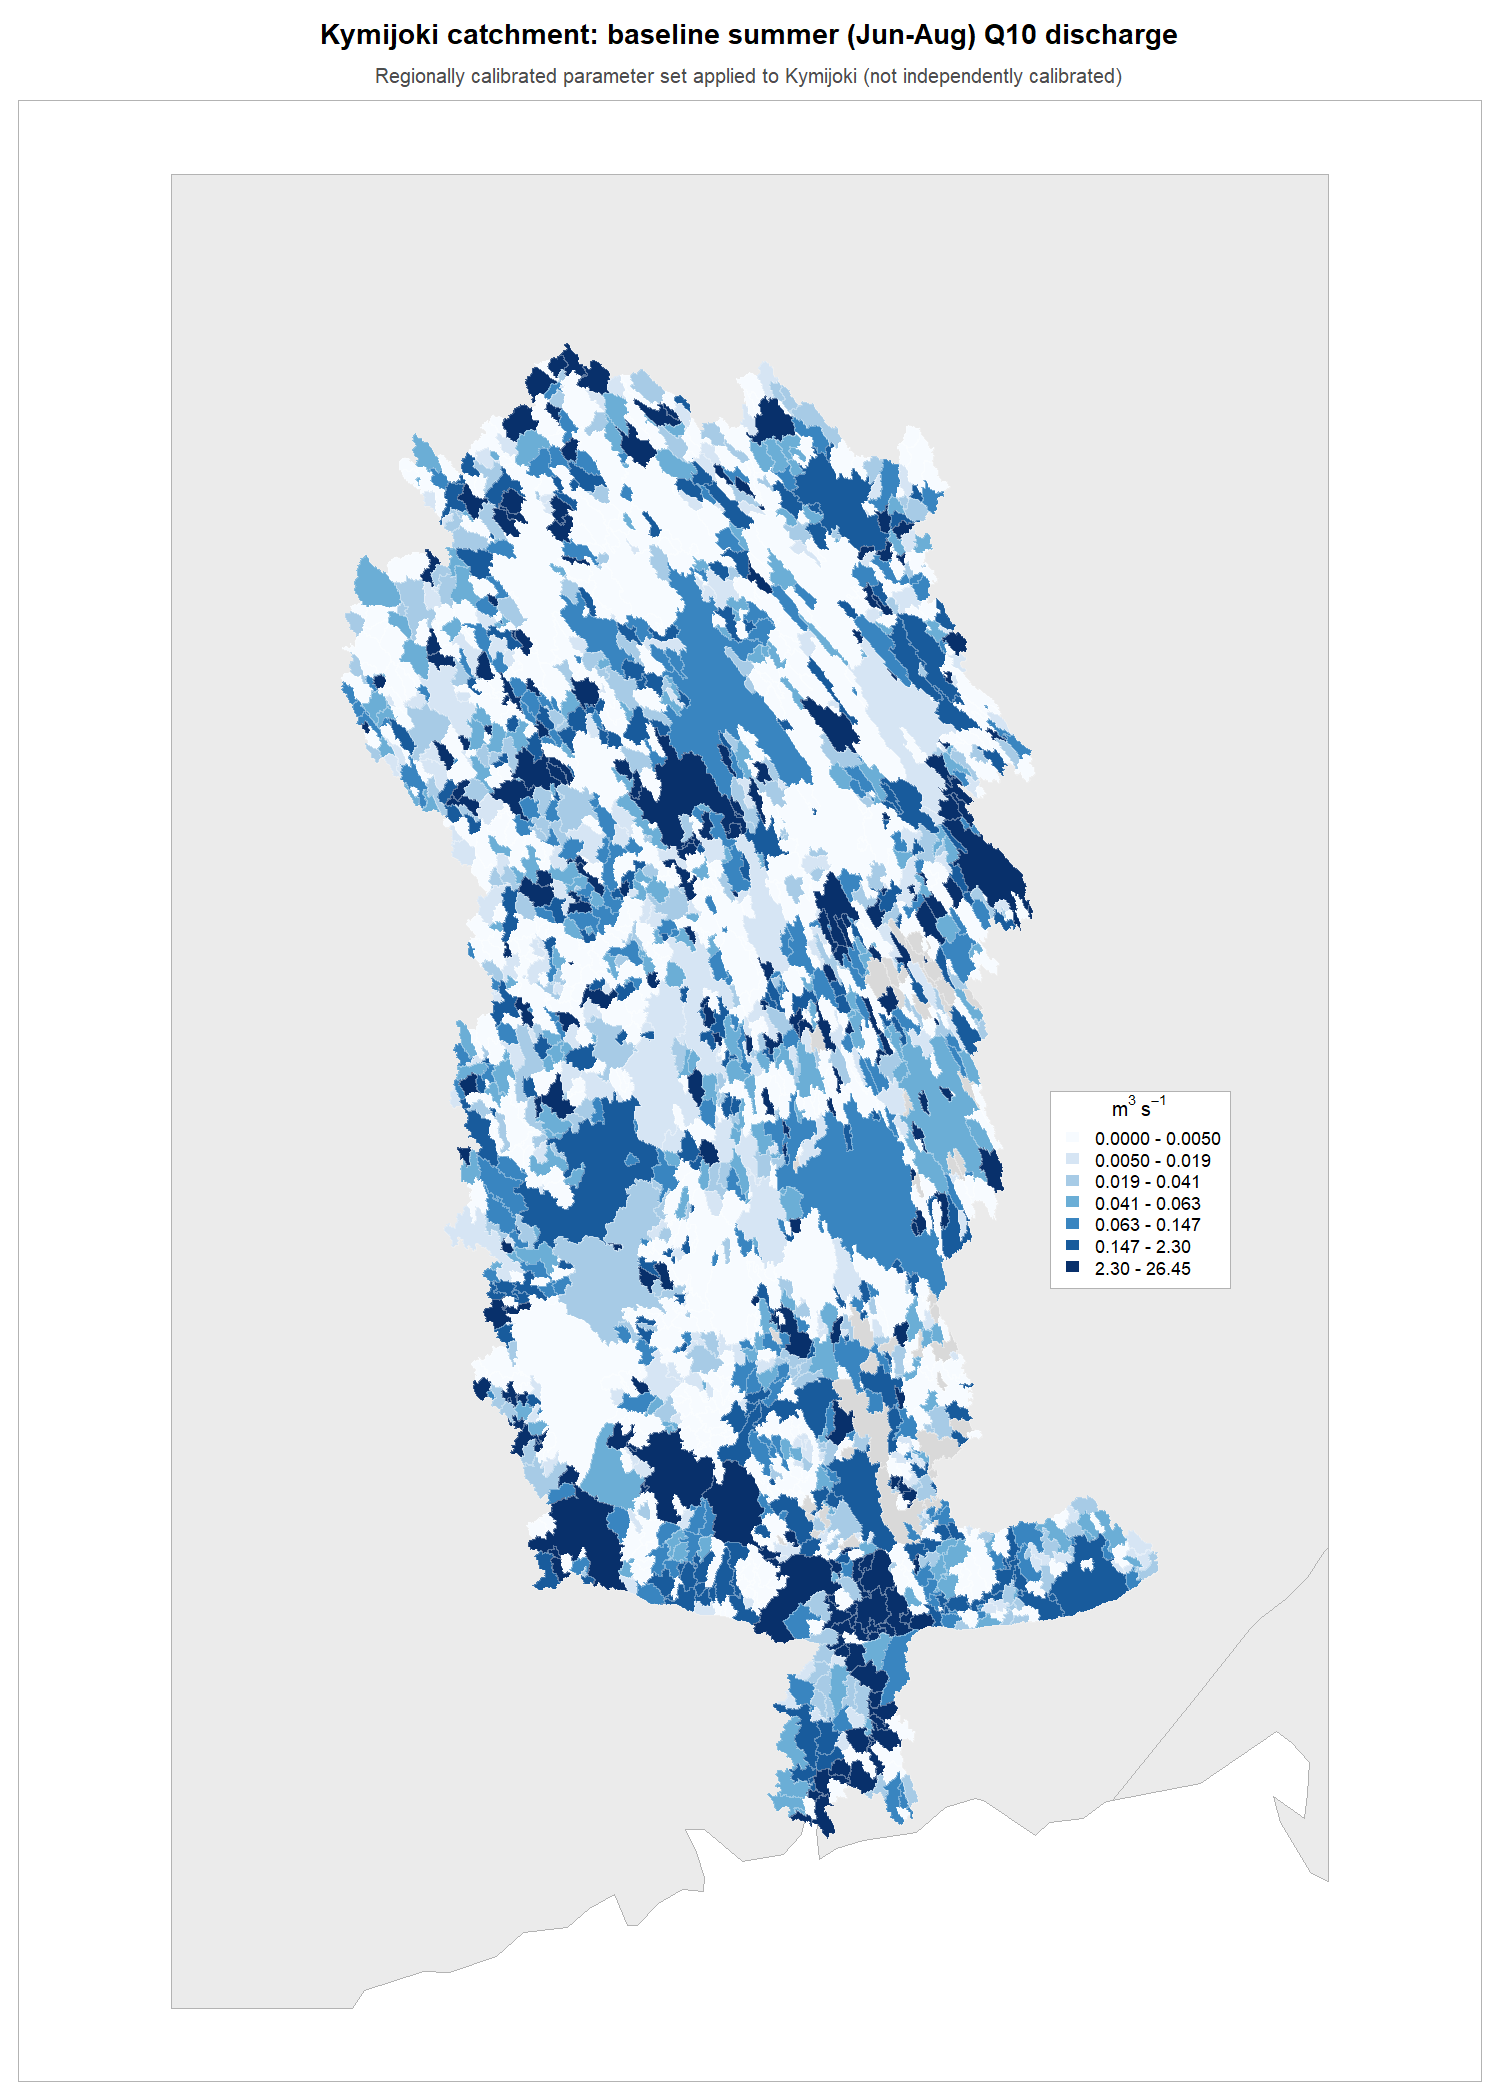
\includegraphics[width=0.55\textwidth]{figures_manuscript/figB1_kymijoki_baseline_summer_q10}
\caption{Kymijoki catchment: baseline summer (June--August) Q10 discharge (m$^3$\,s$^{-1}$) across 2,073 subcatchments, using the regionally calibrated parameter set transferred from the 27 primary study catchments (Kymijoki was not itself part of the calibration domain; see \ref{app:kymijoki}). Colour scale uses quantile-based classification, as in Figure~\ref{fig:seasonal_maps}; light blue = low, dark blue = high discharge; grey = no data (excluded degenerate polygons).}
\label{fig:kymijoki_baseline}
\end{figure}

\subsection{Climate change scenario}

Under the SSP2-4.5 climate scenario, summer Q10 in Kymijoki decreases by a regional median of 37.4\% (P10: $-$76.6\%, P90: $-$13.2\%), with 98.3\% of subcatchments showing a decrease --- consistent in direction with, but larger in magnitude than, the 24.4\% median decrease found across the 27 primary catchments (Section~3.3). Winter Q10 increases by a median of 38.5\%, with 79.2\% of subcatchments showing an increase, mirroring the snow-to-rain shift identified in the primary analysis. The urban growth scenario has a negligible effect in Kymijoki (median summer Q10 change of 0\%, with only 17.1\% of subcatchments showing any decrease and none showing an increase), consistent with the catchment's predominantly forested and rural land cover; the combined scenario is accordingly almost identical to the climate-only scenario (median summer Q10 change $-$37.4\%).

\begin{figure}[htbp]
\centering
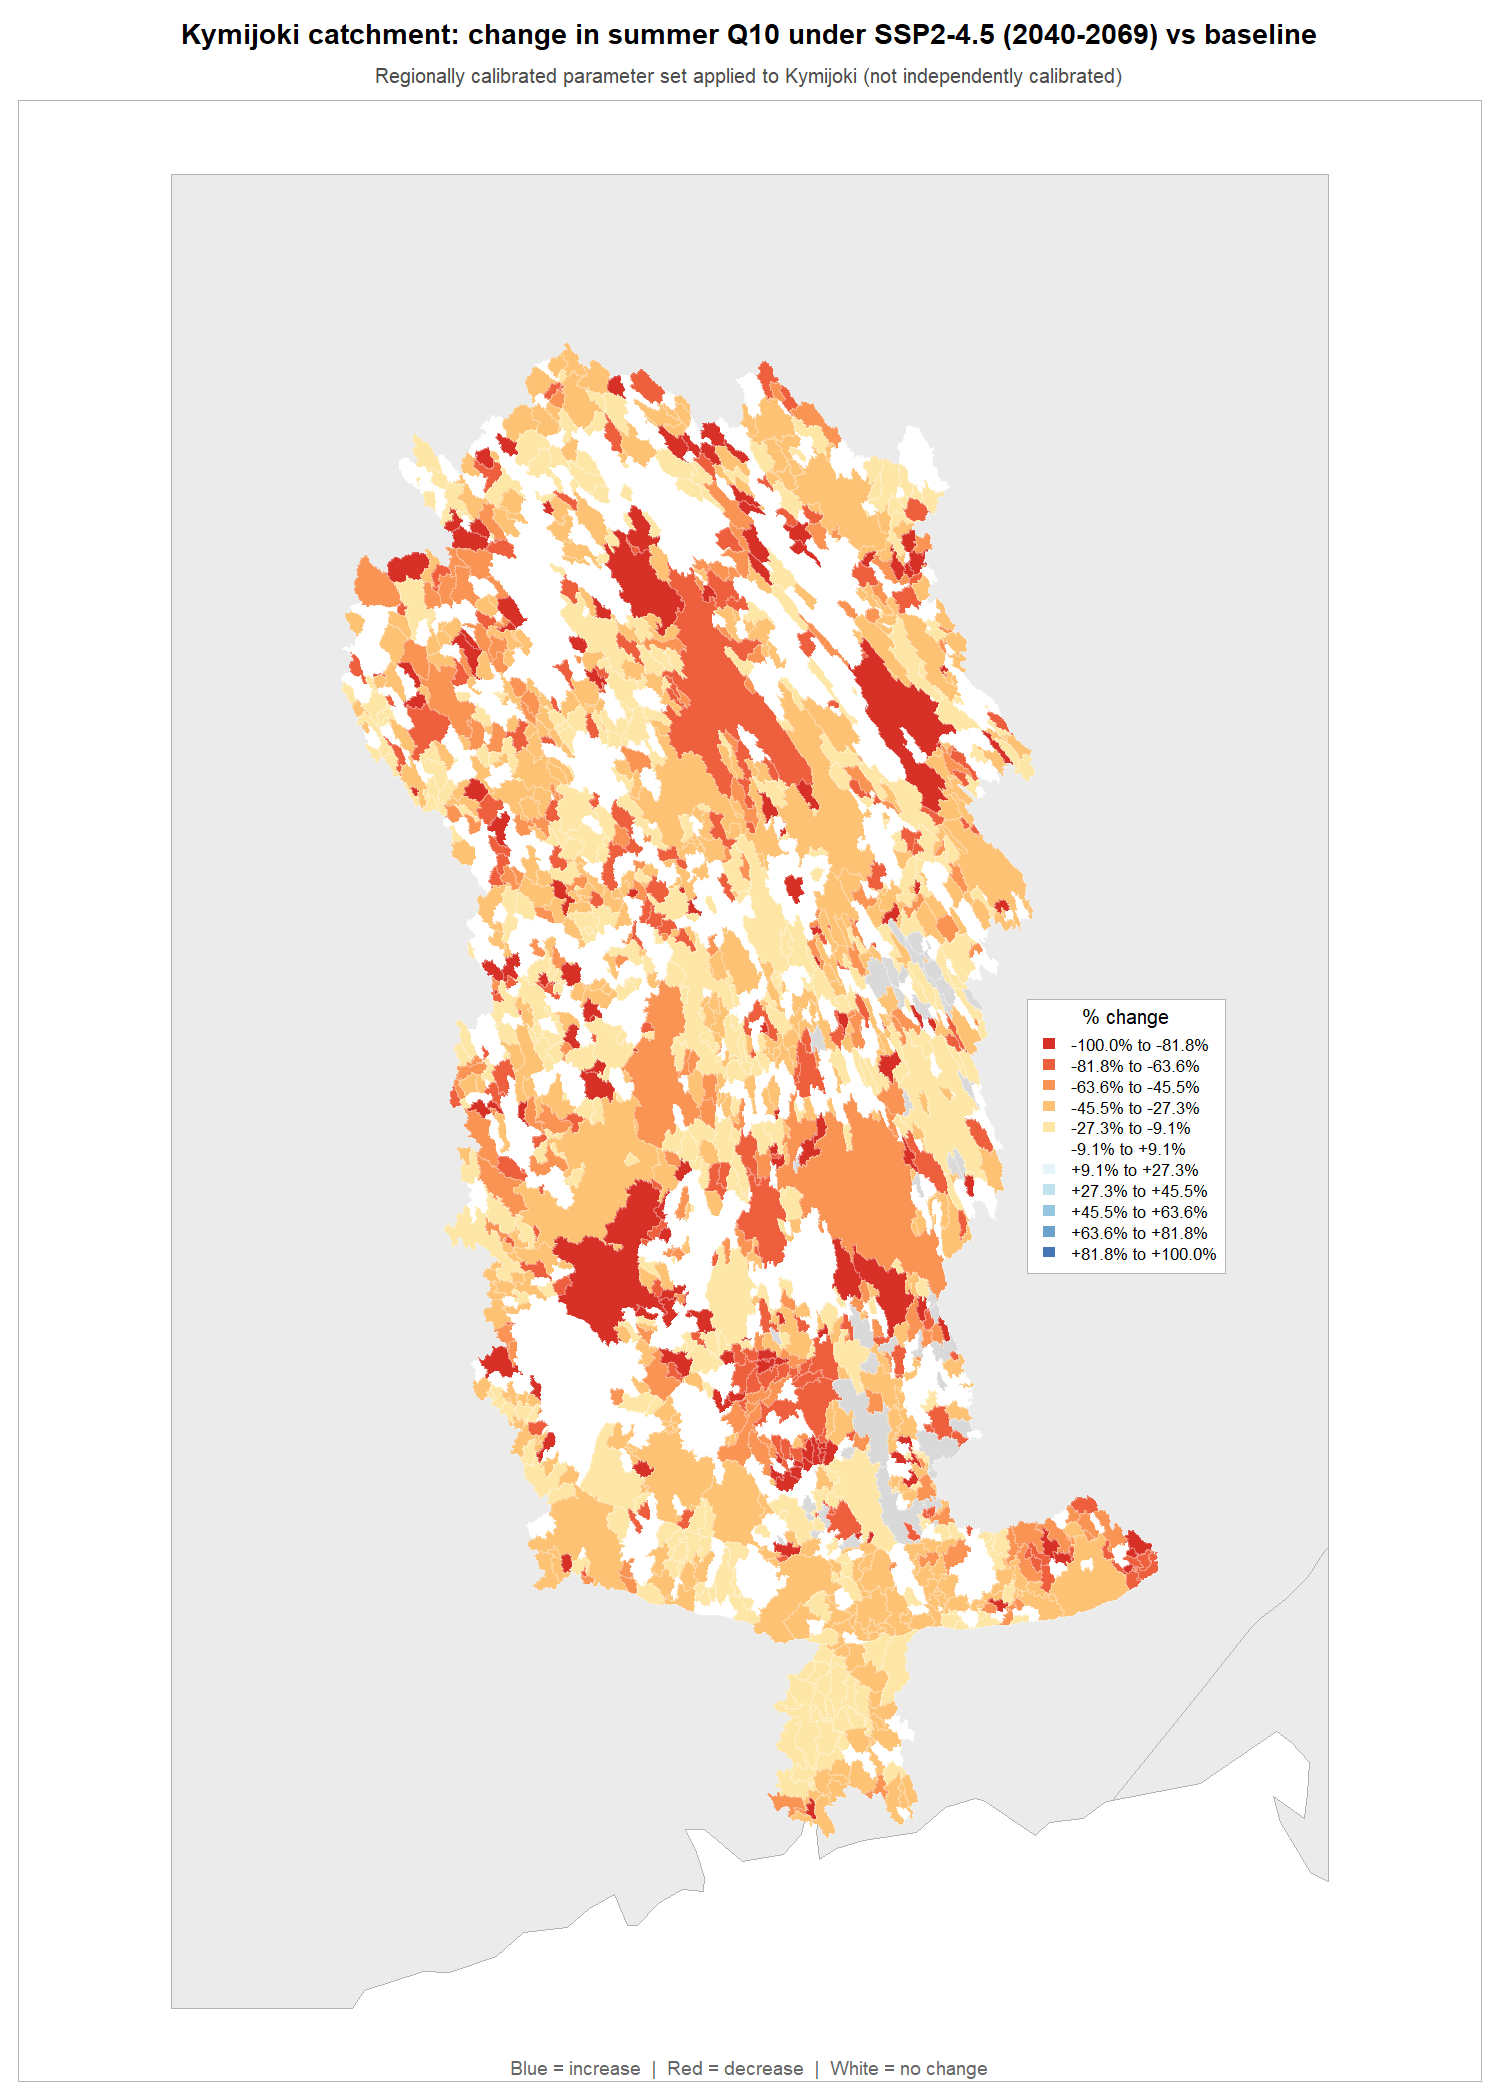
\includegraphics[width=0.55\textwidth]{figures_manuscript/figB2_kymijoki_climate_summer_q10_delta}
\caption{Kymijoki catchment: percentage change in summer Q10 from baseline under the climate change scenario (SSP2-4.5, 2040--2069), using the transferred regional parameter set (see \ref{app:kymijoki}). Red = decrease; blue = increase; white = no change; grey = undefined (baseline Q10 = 0) or excluded degenerate polygon. Note the near-universal decrease, more pronounced than in the primary 27-catchment domain (cf.\ Figure~\ref{fig:delta_summer}).}
\label{fig:kymijoki_delta_summer}
\end{figure}

\subsection{Caveats specific to Kymijoki}

Because Kymijoki was not part of the calibration domain, these results carry additional uncertainty beyond that already discussed for the 27 primary catchments (Section~4.6). In particular: (i) the transferred parameter set may not adequately represent the very large lakes and reservoirs that dominate storage and routing in this basin, several of which are substantially larger than any lake in the 27 primary catchments; (ii) the ``natural'' flows reported here will differ, in places substantially, from what is actually observed at any point on the regulated main stem, where hydropower operators control releases according to energy demand, flood management, and minimum flow commitments rather than natural hydrological variability; and (iii) subcatchment-level detail away from the main stem --- on tributaries that are not themselves regulated --- is more likely to reflect genuine natural flow conditions and may be of more direct practical relevance for siting purposes than main-stem values. For these reasons, the Kymijoki results presented here should be treated as an indicative, first-order estimate of natural water availability rather than a validated assessment, and are reported separately from the primary study's regional statistics (Section~3) for this reason.

\end{document}
